\RequirePackage{fix-cm}                                     % Fix font with siunitx
\documentclass[english, a4paper, twoside, openright, 12pt]{report}	% Document type
%\usepackage{emptypage}                                      % Empty pages
\RequirePackage[l2tabu, orthodox]{nag}                      % Detect deprecated packages, commands, etc.
\usepackage[all,error]{onlyamsmath}                         % Error on deprecated math commands like $$ $$.
\AtBeginDocument{\catcode`$=3 }                             % Workaround for tikz
\usepackage{fixmath}                                        % Fix non ISO behaviour with capital greek letters
%\usepackage{refcheck}                                       % Display warning on unused references
%\ignoreunlbld                                               % Ignore equations in refcheck
\usepackage{todonotes}                                      % TODO

\usepackage{lipsum}                                         % Generate random text (ONLY FOR TEST PURPOSES)


% --- Mathematical packages ---
\usepackage{amsmath}                                        % Math
\usepackage{amsthm}                                         % Theorems and proofs
\usepackage{amssymb}                                        % Math symbols
\usepackage{bm}												% Bold math
\usepackage[per-mode=fraction,
            exponent-product=\cdot,
            separate-uncertainty=true
           ]{siunitx}                                       % Physical units
%\usepackage{mathtools}                                      % Math tools


% --- Typographical packages ---
% - Bases -
\usepackage[utf8]{inputenc}                                 % UTF-8 Encoding
\usepackage[T1]{fontenc}                                    % Font encoding
\usepackage{babel}                                          % Translation
\usepackage[babel]{csquotes}                                % Quotes
\usepackage{comment}                                        % Comments
% - Font -
\usepackage{newtxtext,newtxmath}                            % Times font
\usepackage[toctitles,compact,explicit]{titlesec}           % Custom chapter headings
\usepackage{microtype}                                      % Typographical improvements
\usepackage{ellipsis}                                       % Whitespace correction
% - Shape -
\usepackage[hyphens]{url}                                   % Hyphens in URLs
\usepackage{varioref}
\usepackage{hyperref}                                       % Clickable references
\usepackage[noabbrev]{cleveref}
\usepackage[backend=biber,					% Backend
            bibencoding=utf8,				% File encoding (BibTex = ASCII, Biber = UTF8)
            bibstyle=authoryear,		    % Reference style
            citestyle=authoryear,           % Citation style
            bibwarn=true,                   % Enable warnings
            natbib=true,					% Natbib compatibility
            maxcitenames=2,					% Cite : > 2 name = et al.
            maxbibnames=99,					% Bib  : show all names
            sortcites=true,					% Sorting
            block=space,					% Space between citations
            giveninits=true,				% Compress first names
            uniquename=init,				% Compatible with 'giveninits=true'
            isbn=false,                     % Disable ISBN
            doi=false                       % Disable DOI
           ]{biblatex}
\usepackage{fancyhdr}                                       % Custom head- and foot-lines
\usepackage{setspace}                                       % Spacing between lines
\usepackage[titles]{tocloft}                                % Spacing in table of contents
%\usepackage{abstract}                                       % Abstract
\usepackage{geometry}                                       % Geometry of a page

% --- Graphical packages ---
\usepackage{float}                                          % float environment settings
\usepackage{graphicx}                                       % Figures
\usepackage{caption}                                        % Figures and captions
\usepackage{subcaption}                                     % Figures and captions (side-by-side)
\usepackage{booktabs}                                       % Improved tables
\usepackage{multirow}                                       % Multirow


\usepackage{pbox}
% Disable underfull box warnings when breaking URLs
\usepackage{etoolbox}
\apptocmd{\sloppy}{\hbadness 10000\relax}{}{}


% The literature file
\addbibresource{tex/literature.bib}





% --- Style ---



% Fix für strange spacing in left right environments
\let\originalleft\left
\let\originalright\right
\renewcommand{\left}{\mathopen{}\mathclose\bgroup\originalleft}
\renewcommand{\right}{\aftergroup\egroup\originalright}



% Penalties for paragrpahs starting or ending at a page
%\clubpenalty         = 10000
%\widowpenalty        = 10000
%\displaywidowpenalty = 10000


% The geometry of the page
\newlength{\bindingOffset}
\setlength{\bindingOffset}{0mm}

\geometry{a4paper,
    	  twoside,
          bindingoffset = \bindingOffset,
          top = 35mm, bottom = 35mm,
          inner = 25mm, outer = 25mm - \bindingOffset,
          headheight = 15pt,
          headsep = 15pt,
          footskip = \headheight + \headsep + 3pt
          %showframe
         }


% Spacing between lines
\setstretch{1.125}



% Spacing of paragraphs
\parskip   = 0.5\baselineskip \advance\parskip by 0pt plus 2pt
\parindent = 0pt


% Column separtation size
\setlength{\columnsep}{0.05\textwidth}


% Bibligraphy item separation size
\setlength\bibitemsep{1.5\itemsep}




% Head- and foot-lines
\fancypagestyle{plain}
{
    \fancyhf{}
    \fancyfoot[C]{\thepage}
    \renewcommand{\headrulewidth}{0pt}
    \renewcommand{\footrulewidth}{0.4pt}
}

\fancypagestyle{plainline}
{
    \fancyhf{}
    \fancyfoot[C]{\thepage}
    \renewcommand{\headrulewidth}{0.4pt}
    \renewcommand{\footrulewidth}{0.4pt}
}

\pagestyle{fancy}
\fancyhf{}
\fancyhead[CE]{\rightmark}
\fancyhead[CO]{\leftmark}
\fancyfoot[C]{\thepage}
\renewcommand{\headrulewidth}{0.4pt}
\renewcommand{\footrulewidth}{0.4pt}




% Empty pages
\makeatletter
\def\cleardoublepage{\clearpage%
    \if@twoside
    \ifodd\c@page\else
        \begin{minipage}[c][\textheight][c]{\textwidth}
            \begin{center}
                %This page intentionally left blank.
            \end{center}
        \end{minipage}
        \vfill
        \thispagestyle{plainline}
        \newpage
    \if@twocolumn\hbox{}\newpage\fi
    \fi
    \fi
}
\makeatother





% Chapter headings
\newlength\chapnumb
\setlength\chapnumb{4cm}

\newlength\chapnumbfontsize
\setlength\chapnumbfontsize{80pt}

\titleformat{\chapter}[block]
{\normalfont %\sffamily
}{}{0pt}
{\parbox[b]{\chapnumb}{%
        \fontsize{\chapnumbfontsize}{0}\selectfont\thechapter}%
    \parbox[b]{\dimexpr\textwidth-\chapnumb\relax}{%
        \raggedleft%
        \hfill{\Huge\textbf{#1}}\\
        \rule{\dimexpr\textwidth-\chapnumb\relax}{0.4pt}}}
\titleformat{name=\chapter,numberless}[block]
{\normalfont %\sffamily
}{}{0pt}
{\parbox[b]{\chapnumb}{%
        \fontsize{\chapnumbfontsize}{0}\selectfont\color{white}0}%
    \hspace{-\chapnumb}\parbox[b]{\dimexpr\textwidth\relax}{%
        \raggedleft%
        \hfill{\Huge\textbf{#1}}\\
        \rule{\dimexpr\textwidth\relax}{0.4pt}}}




% Hyperref settings
\hypersetup{colorlinks    = true,                                                                % Color links
            linkcolor     = black      , citecolor = black, filecolor = black, urlcolor = black, % Link ad URL colors
            pdfauthor     = {\@author} , pdftitle = {\@title},                                   % Author und Title
            pdfpagelayout = TwoPageRight%                                                        % double-sided view
           }


% Only show contents up to section level
\setcounter{tocdepth}{1}


% Spacing in table of contents
\setlength{\cftbeforechapskip}{4.75mm}
\setlength{\cftbeforesecskip}{-1.5mm}
\setlength{\cftbeforesubsecskip}{-2.0mm}


% Force table to be set at given position
\restylefloat{table}

% Spacing in tables
\newcommand{\setArraystrech}[1]{\renewcommand{\arraystretch}{#1}}


% SI settings
\sisetup{
    locale = DE,
    binary-units = true,
    output-decimal-marker = {,},
    group-digits = true,
    group-separator = {\,},
    per-mode = symbol
}
\DeclareSIUnit{\bit}{Bit}


% Subcaption settings
\captionsetup{subrefformat=parens}


% Fix comment environment
\renewenvironment{comment}{}{}




% --- Macros ---

% Blank line
\newcommand{\blankline}{\vspace{\baselineskip}}


% Intervals
\newcommand{\interval}[2]{\ensuremath{[ #1 \,, #2 ]}}


% Norm and absolute value
\newcommand{\norm}[1]{\ensuremath{\left\Vert#1\right\Vert}}
\newcommand{\abs}[1]{\ensuremath{\left\vert#1\right\vert}}


% Dot product and cross product
\newcommand{\dynamicvert}[1]{\,\left\vert\vphantom{#1}\right.}
\newcommand{\dotproduct}[2]{\ensuremath{\left\langle\,#1\,\middle\vert\,#2\,\right\rangle}}
\newcommand{\crossproduct}[2]{\ensuremath{#1\times#2}}



\newcommand{\order}[1]{\mathcal{O}\left(#1\right)}

\newcommand{\expectation}[1]{\mathbb{E}\left[#1\right]}
\newcommand{\deviation}[1]{\mathbb{D}\left[#1\right]}
\newcommand{\variance}[1]{\mathbb{D}^2\left[#1\right]}




% argmin
\DeclareMathOperator*{\argmin}{arg\,min}
\DeclareMathOperator*{\argmax}{arg\,max}


% sign
\newcommand{\sign}[1]{\mathrm{sign}\left(#1\right)}


% XOR
\newcommand{\xor}{\mathbin{\oplus}}


% Functions with brackets
\renewcommand{\min}[1]{\mathrm{min}\left(#1\right)}
\renewcommand{\max}[1]{\mathrm{max}\left(#1\right)}
\renewcommand{\tan}[1]{\mathrm{tan}\left(#1\right)}
\newcommand{\logarithm}[2]{\mathrm{log}_{#1}\left(#2\right)}

\newcommand{\nn}[2][]{\underset{#1}{\mathrm{nn}}\left(#2\right)}

\newcommand{\ME}[1]{\mathrm{ME}\left(#1\right)}
\newcommand{\RMSE}[1]{\mathrm{RMSE}\left(#1\right)}
\newcommand{\NME}[1]{\mathrm{NME}\left(#1\right)}
\newcommand{\NRMSE}[1]{\mathrm{NRMSE}\left(#1\right)}
\newcommand{\PSNR}[1]{\mathrm{PSNR}\left(#1\right)}
\newcommand{\BB}[1]{\mathrm{BB}\left(#1\right)}


% Plus-equal
\newcommand{\pluseq}{\mathrel{+}=}


% Tilde in math mode
\newcommand{\mathtilde}{{\raise.17ex\hbox{$\scriptstyle\mathtt{\sim}$}}}



% Alignment in algorithms
\newcommand{\alignto}[2]{\mathrlap{#2}\phantom{#1}}





% Mathematical blocks
\newtheorem{lemma}{Lemma}[chapter]
\newtheorem{theorem}{Theorem}[chapter]
\newtheorem{definition}{Definition}[chapter]
\newtheorem{corollary}{Corollary}[chapter]


% Gradient, Divergenz and Laplace
\DeclareMathOperator{\gradient}{\nabla}
\DeclareMathOperator{\divergence}{div}
\DeclareMathOperator{\laplacian}{\Delta}


% Vector with an arrow above
\let\oldvec\vec
\newcommand{\vecarrow}[1]{\oldvec{#1}}

% Vector and Matrix macros		
\renewcommand{\vec}[1]{\bm{#1}}
\newcommand{\mat}[1]{\bm{#1}}
\newcommand{\set}[1]{\mathcal{#1}}
\newcommand{\neighborhood}[1]{\mathcal{N}(#1)}

% More intutive macros for set operations
\newcommand{\intersect}[0]{\cap}
\newcommand{\union}[0]{\cup}
\newcommand{\difference}[0]{\,\backslash\,}

\newcommand{\bigintersect}[0]{\bigcap}
\newcommand{\bigunion}[0]{\bigcup}

% Probability
\newcommand{\probability}[1]{\mathrm{Pr}(#1)}
\newcommand{\probabilitygiven}[2]{\mathrm{Pr}(#1\mid#2)}


\newcommand{\transposed}{\top}


\newcommand{\evalat}[2]{\left.\kern-\nulldelimiterspace#1\right|_{\substack{#2}}}


\newcommand{\const}{\mathrm{const}}


% Table stuff
\newcolumntype{L}[1]{>{\raggedright\arraybackslash}m{#1}}
\newcolumntype{C}[1]{>{\centering\arraybackslash}m{#1}}
\newcolumntype{R}[1]{>{\raggedleft\arraybackslash}m{#1}}

% Colors
\definecolor{burgundy}{rgb}{0.5, 0.0, 0.13}
\definecolor{cadmiumgreen}{rgb}{0.0, 0.42, 0.24}
\definecolor{bronze}{rgb}{0.8, 0.5, 0.2}

\newcommand{\im}[1]{{\color{blue}#1}}
\newcommand{\sm}[1]{{\color{red}#1}}

\newcommand*\rot[1]{\rotatebox{90}{#1}}


\graphicspath{{./figures/}}



% % % % % % % % % % % % % % % % % % % % % % % % % % % % % % % % % % % % % % % % % % % % % % % % %

\newcommand{\im}[1]{{\color{blue}#1}}

\newcommand{\thesisType}{Thesis}

\title{Accelerations for Training and Rendering Neural Reflectance and Radiance Fields}

\author{Ilia Mazlov}

\newcommand{\firstReviewer}{Prof. Dr. Reinhard Klein}
\newcommand{\secondReviewer}{Dr. Michael Weinmann}

\date{\today}


% Generate author and title
\makeatletter

% % % % % % % % % % % % % % % % % % % % % % % % % % % % % % % % % % % % % % % % % % % % % % % % %



\begin{document}
    % Start with roman page numbers
    \pagenumbering{Roman}


	% Title page
	


{
	% New spacing
	\onehalfspacing
	
    \setlength{\parskip}{0cm}
	
	\begin{titlepage}
        %\fbox{
        \begin{minipage}[c][0.3\textheight][t]{\textwidth}
            %\fbox{
            \begin{minipage}[c][0.05\textheight][t]{\textwidth}
                
                
                % Kind of thesis
                \begin{center}
                    \Large\textsc{\thesisType}
                \end{center}
                
                
            \end{minipage}
            %}
            \par\nointerlineskip % remove space between boxes
            %\fbox{
            \begin{minipage}[c][0.20\textheight][c]{\textwidth}
                
                % Use second minipage to force rule to be inside the first minipage
                \begin{minipage}[c][0.20\textheight][c]{\textwidth}
                    \rule{\linewidth}{0.4pt}
                    %\fbox{
                    \begin{center}
                        \LARGE\@title
                    \end{center}
                    %}
                    \rule{\linewidth}{0.4pt}
                \end{minipage}
                
            \end{minipage}
            %}
            \par\nointerlineskip % remove space between boxes
            %\fbox{
            \begin{minipage}[c][0.05\textheight][b]{\textwidth}
                
                
                % Author
                \begin{center}
                    \Large\@author
                \end{center}
                
                
            \end{minipage}
            %}
            \par\nointerlineskip % remove space between boxes
        \end{minipage}
        \par\nointerlineskip % remove space between boxes
        %}
        %\fbox{
        \begin{minipage}[c][0.4\textheight][c]{\textwidth}
            
            
            \begin{center}
               
\includegraphics[height = 0.275\textheight, keepaspectratio]{logo_white.jpg}
            \end{center}
            
            
        \end{minipage}
        \par\nointerlineskip % remove space between boxes
        %}
        %\fbox{
		\begin{minipage}[c][0.3\textheight][t]{\textwidth}
            %\fbox{
            \begin{minipage}[c][0.1\textheight][t]{\textwidth}
                
                
                \begin{center}
        			% Institute
        			\textsc{Institute of Computer Science II - Computer Graphics \\
        					University of Bonn} \\[1.5cm]
                \end{center}
                
                
   			\end{minipage}
   			%}
            \par\nointerlineskip % remove space between boxes
            %\fbox{
            \begin{minipage}[c][0.1\textheight][c]{\textwidth}
                
                
                \begin{center}
                    % Reviewer
                    \begin{tabular}{rl}
                        First Reviewer:   & \firstReviewer \\
                        Second Reviewer:  & \secondReviewer \\
                    \end{tabular}
                \end{center}
                
                
            \end{minipage}
            %}
            \par\nointerlineskip % remove space between boxes
            %\fbox{
            \begin{minipage}[c][0.1\textheight][b]{\textwidth}
                
                
                \begin{center}
                    % Date
                    \large\@date
                \end{center}
                
                
            \end{minipage}
            %}
            \par\nointerlineskip % remove space between boxes
		\end{minipage}
    	%}
	\end{titlepage}
}


% back page blank
\cleardoublepage






    % Statutory declaration
	


{
    %\thispagestyle{empty}
    
    
    \begin{minipage}[c][\textheight][c]{\textwidth}
        \begin{center}
            \huge{Statutory Declaration}
        \end{center}
        
        \vspace*{1.5cm}
        
        I declare that I have developed and written the enclosed Thesis completely by myself, and have not used sources or means without declaration in the text. Any thoughts from others or literal quotations are clearly marked. The Thesis was not used in the same or in a similar version to achieve an academic grading or is being published elsewhere.
        
        \vspace*{2cm}
        
        \begin{center}
            \begin{tabular}{cp{2.5cm}c}
                \hspace{5cm}   && \hspace{5cm} \\
                \cline{1-1}\cline{3-3}
                \addlinespace
                Location, Date && Signature
            \end{tabular}
        \end{center}
    \end{minipage}
    

}


% Rückseite leer
\cleardoublepage






	% Abstract / summary
	

% Abstract
\chapter*{Summary}
\label{sec:summary}
%\addcontentsline{toc}{chapter}{Zusammenfassung}

% \im{condense}

Photo-realistic scene reconstruction under novel viewing and illumination conditions
is a challenging long-standing problem in computer graphics.
Recent studies in this field have shown the applicability of deep neural networks
to learn an implicit neural representation of the scene
containing both geometric and appearance information about the scene.

Most works focus on extracting radiance fields under the static illumination of the scene.
\cite{mildenhall2020nerf} presented the state-of-the-art approach NeRF,
which learns continuous volumetric scene representation from the set of known 2D views.
This allows to reconstruct the learned scene from the novel viewpoints,
however, the proposed approach suffers from inefficiency.
To improve NeRF's performance \cite{liu2021neural} show the application of octrees
to learn Neural Sparse Voxel Fields (NSVF) that achieve up to 10 times better performance.

However, learned with NSVF radiance fields are still not implying any light interaction that allows
to model light-dependent effects and reconstruct the scene under novel illumination conditions.
\cite{bi2020neural} propose Neural Reflectance Fields (NRF)
that considers a single non-static point light illumination on the scene
and implies additional light rays sampling, which drastically increases method complexity.

In this work, the performance limitation is addressed and several methods
that allow increasing NRF's efficiency are offered.
Explicit schemes \textit{ExCol} and \textit{ExBF} are meant to accelerate NRF approach
using voxel octree structure, similarly to NSVF approach.
Explicit scheme \textit{ExVA} offers the in-voxel approximation,
which makes the \textit{ExBF} method more practical.
Another \textit{ImNRF} method is based on the original NSVF approach
and implies learning an implicit neural reflectance representation of the scene.






% \lipsum[1-2]




    % Acknowledgement
    

% Abstract
\chapter*{Acknowledgments}
\label{sec:acknowledgement}
%\addcontentsline{toc}{chapter}{\nameref{sec:acknowledgement}}

I want to thank ...



	% Table of contents
	\tableofcontents

	%\newpage

    % List of figures
	%\listoffigures

    % List of tables
	%\listoftables

    % List of algorithms
    %\listofalgorithms

    %\newpage


    % Regular page numbers
    \cleardoublepage
    \pagenumbering{arabic}


    % % % % % % % % % % % % % % % % % % % % % % % % % % % % % % % % % % % % % % % % % % % % % % % % % % % % % % % % % % % % % % % %

    \chapter{Introduction}
\label{chap:introduction}

% kind of problem statement in introduction
% positions required, but meshroom can be used
% scenes with highly specular objects trains better using log-transform
% discussion part: background color problem
% layer depth for NSVF can be way more shallow since voxel features
% assuming single(!) point(!) light only
% inverseCDF sampling for NSVF
% discrete regularization - noise to sigma field
% calculating normals from sigma and directly outputing normals


% light attenuation + light as learnable parameter (as there barely exist the ground truth value for real datasets)
% different sigma in voxel strategies for inVoxelApproximation


The task of reconstructing a real 3D scene from a set of 2D captured images
and modeling it under novel viewing and lighting conditions
is a long-standing problem in computer graphics and vision.
Possible complex scene geometries along with numerous appearance properties
make this task a tremendously challenging problem.
The real-world scenes contain a descent amount of complications
that can come from both the environment (e.g. illumination is not completely static)
and from the capturing hardware (e.g. distortions in camera lenses, low dynamic range (LDR) images).

The applications of realistic rendering include diverse fields,
such as visualization, animation, virtual and augmented reality, visual effects,
and even computer vision and robot navigation.

% \im{image here similar to in NeRF with the pipeline}

% Not very long about very basics
% \subsection{\{Rendering equation\} \im{or/and radiometry?}}
% \begin{enumerate}
%     %\item Color space \im{?}
%     \item LDR/HDR
%     \item Rendering equation
%     \item Transfer equation
%     \item (simple) volume rendering
%     \item BSSRDF + Reflection Models
% \end{enumerate}
% \sm{Not sure how relevant that is. Maybe put this in a subsection later for NeRF? Lowest priority for now.}

This task was traditionally addressed to the image-based rendering systems,
which use vision-based scene geometry together with the image-based view interpolation \cite{shumandkang2000}.
However, recent works in this field make use of deep neural networks
in order to learn implicit "neural" scene representation,
containing both geometric and appearance information. \cite{tewari2020state}

\cite{mildenhall2020nerf} presented a state-of-the-art approach,
which uses deep neural network as an implicit continuous volumetric scene representation.
In the core of this method lies the volume ray casting technique \cite{drebin1988volume},
which implies such volume processes as absorption and emission
while not accounting for scattering.
View rays are traced through the 2D captures of the scene,
sampled in a 3D space and then processed with neural network,
which predicts the volume density and color value at the given spatial point under a given viewing direction.
% These samples along the ray are used to estimate the rendering integral.
These samples along the ray are used to predict volume density and color value,
which are then gathered via alpha-compositing process.
This approach has quickly become a starting point for lots of other works \cite{liu2021neural, garbin2021fastnerf, reiser2021kilonerf, yu2021plenoctrees, rebain2020derf, lindell2021autoint}.
However, the main limitation for most of them is the lack of light interaction,
which disables the capabilities for rendering the scene under the novel light conditions.

\cite{bi2020neural} propose the NRF approach
that removes this limitation by reformulating the rendering equation in a way
that it accounts for the \textit{light transmittance},
i.e. the accumulated volume transmittance along corresponding light rays.
This approach only considers a single (but not static) point light source located on the scene.
However, the proposed implementation is only practical for one specific case
when the light source is co-located with the camera.
Although, this approach is already able to generalize for the relighting of the scene,
the predictions are still affected by a very sparse light-view space sampling
as there are only coincident light and view rays in the training dataset
(e.g. the model never deals with shadows on the training sample images).


% \section{Goal of the Thesis}
The goal of this thesis is to develop a solution
that is able to model scene geometry and appearance with view- and light-dependant effects
implying both co-located and non-colocated light sources.
This is done by utilizing the usage of neural sparse voxel fields (NSVF) \cite{liu2021neural}
with such a problem formulation that considers a single point light source illumination \cite{bi2020neural}.
This method is called \textit{ExCol} (Explicit Colocated) and is only capable
to be processed within the co-located setting as in NRF approach.

In order to extend this setup for the non-colocated light setting, the \textit{ExBF} (Explicit Brute-Force) method is proposed,
which traces and samples light rays for each of the view sample points to calculate light transmittance values.
However, this approach is unrealistically slow and memory-demanding,
which makes it impractical.

It is proposed to solve this problem by an approximation scheme \textit{ExVA} (Explicit with in-Voxel Approximation),
which leverages the usage of voxel octree structure
and approximates light transmittance by the distance that light ray has travelled inside voxels.
This method seems to be able to perform at the same level of quality as the initial \textit{ExBF} scheme,
though drastically outperforming it in terms of efficiency.

\im{say about ImNRF}

To summarize, the contributions of this work are:
\begin{enumerate}
    \item An acceleration technique \textit{ExCol} for the NRF approach
    based on Neural Sparce Voxel Fields
    \item The approximation scheme \textit{ExVA}
    for the generalization \textit{ExBF} of proposed \textit{ExCol}
    that achieves comparable results with only a minor overhead
    \item The implicit scheme \textit{ImNRF} \im{continue}
    % \item The implementation of all of the listed schemes: \textit{ExCol}, \textit{ExBF} and \textit{ExVA}
    \item Extension from LDR to HDR data
\end{enumerate}



% \section{Outline}
% In Chapter 2 related background along with already existing methods are described.

% Chapter 3 is dedicated to the proposed method.

% Chapter 4 describes and analyses the experiments and the results.


% \textit{Another difficulty is the low dynamic range (LDR) images
% that usually come as a result of capturing real-world scenes.
% LDR images can be under- or over-exposured, which definitely makes the problem harder.
% The high dynamic range (HDR) images can be achieved
% by capturing series of LR images with different exposure values
% and then blending them together into a single HDR image.
% However, this makes the whole process of retrieving real-world data highly complex. (\im{wanted to include this as 2nd paragraph, but too detailed, isnt it?})}




% This is the Introduction and this is a text citation to \textcite{bestpaper} where this is a citation in parentheses \parencite{bestpaper}.

% \begin{figure}[!ht]
%     \centering
%     \begin{subfigure}[t]{0.485\textwidth}
%         \centering
%         
\includegraphics[height = 0.2\textheight, keepaspectratio]{logo_white.jpg}
%         \caption{The CG logo}
%         \label{fig:logo_sub_1}
%     \end{subfigure}
%     \begin{subfigure}[t]{0.485\textwidth}
%         \centering
%         
\includegraphics[height = 0.2\textheight, keepaspectratio]{logo_white.jpg}
%         \caption{The CG logo again}
%         \label{fig:logo_sub_2}
%     \end{subfigure}
%     \caption{The logo}
%     \label{fig:logo}
% \end{figure}

% So let us reference the logo above.

% cref : \cref{fig:logo} , \cref{fig:logo_sub_1} , \cref{fig:logo_sub_2}

% Cref : \Cref{fig:logo} , \Cref{fig:logo_sub_1} , \Cref{fig:logo_sub_2}


% \blankline
% Or reference the chapter.

% cref : \cref{chap:introduction}

% Cref : \Cref{chap:introduction}


% \lipsum[1]

% \begin{table*}[!htb]
%     \setArraystrech{1.5}
    
%     \centering
%     \caption{A fancy table showing some measured errors.}
%     \label{tab:benchmark}
%     \begin{tabular}{ L{0.2\textwidth}R{0.15\textwidth}R{0.15\textwidth}R{0.15\textwidth}R{0.15\textwidth}}
%     	\toprule
%     	Data sets                                    &   A &   B &   C &   D \\
%     	\addlinespace
%         \midrule
%         seq 1                                        & 0.1 & 0.2 & 0.3 & 0.4 \\
%     	seq 2                                        & 1.5 & 0.3 & 0.7 & 1.0 \\
%     	seq 3                                        & 0.4 & 0.7 & 9.4 & 0.9 \\ \bottomrule
%     \end{tabular}
% \end{table*}

% \lipsum[2]

 % Introduction

    % % % % % % % % % % % % % % % % % % % % % % % % % % % % % % % % % % % % % % % % % % % % % % % % % % % % % % % % % % % % % % % %

    \chapter{Related work}
\label{chap:related_work}

\section{Basic models and knowledge}

Not very long about very basics
Laying out why the following sections are relevant for this work

\subsection{\{Rendering equation\} \im{or/and radiometry?}}
\begin{enumerate}
    %\item Color space \im{?}
    \item LDR/HDR
    \item Rendering equation
    \item Transfer equation
    \item (simple) volume rendering
    \item BSSRDF + Reflection Models
\end{enumerate}

\sm{Not sure how relevant that is. Maybe put this in a subsection later for NeRF? Lowest priority for now.}

\subsection{Camera model}
\begin{enumerate}
    \item Homogenous coordinates
    \item Pinhole camera model
    \item Intrinsics
    \item Extrinsics
    \item Distortion
\end{enumerate}


\section{Neural scene representation}

\sm{sounds like a good listing}

\begin{enumerate}
    \item Explicit/implicit scene representations
    \item Neural Radiance Field (Scene Representation Networks, Local Light Field Fusion ..->.. NeRF)
    \item Positional encoding (Fourier Features Let Networks Learn...) % How it is performed and what for? The background research behind this.
    \item NeRF optimizations (NSVF, FastNeRF, KiloNeRFAutomatic Integration and others)
    \item Rendering under novel lighting conditions (NRF, DRF, Deep Voxels, NeRD, NeRV, NeRFactor etc)
\end{enumerate}


% \lipsum[1-15] % Related work

    % % % % % % % % % % % % % % % % % % % % % % % % % % % % % % % % % % % % % % % % % % % % % % % % % % % % % % % % % % % % % % % %

    \chapter{Method}
\label{chap:method}

In this chapter I first describe techniques that lie in core of the proposed solution.
They then followed by a detailed explanation of the proposed solution.
Finally I give the implementation details and settings.

\section{Neural Radiance Fields}

The Neural Radiance Fields approach (\cite{mildenhall2020nerf}) lies directly in the heart of the proposed solutions.
The continuous 5D function 

\begin{equation}
    \label{eq:nerf_function}
    F : (p,v) \xrightarrow{} (c, \sigma)
\end{equation}

is required to be achieved in order to solve the novel view synthesis problem.
Given the spatial location $p \in \mathbb{R}^3$ and the 2D viewing direction $(\theta, \phi)$ (or its equivalent 3D Cartesian representation $v \in \mathbb{R}^3$),
one has to obtain the RGB color value $c$ and the volume density $\sigma$ at this exact point $p$ under the viewing direction $v$.
To obtain the image of the scene, one can take a pin-hole camera at position $p_0$ and cast rays to the scene: $p(z) = p_0 + z\cdot v$.
The final visible color value $C(p,v)$ can then be evaluated using volume rendering approach \cite{niemeyer2020differentiable}, \cite{Novak18volumeSTAR} along the ray $p$:
\begin{equation}
    C(p,v) = \int_{0}^{\infty} \omega(p(z)) \cdot c(p(z),v) dz,
    \label{eq:rendering_equation}
\end{equation}
$\omega(p(z))$ is a probability weight function
\begin{equation}
    \omega(p(z)) = \tau_c(p(z)) \sigma(p(z)),
\end{equation}
where $\tau_c(p(z)) = e^{\int_0^z \sigma(p(s)) ds}$ denotes the accumulated transmittance along the ray up to the point $p(z)$, $\sigma(p(z))$ is the volume density at point $p(z)$ and the probability property is held: $\int_0^\infty \omega(p(z))dz = 1$

\begin{figure}[t]
    \centering
    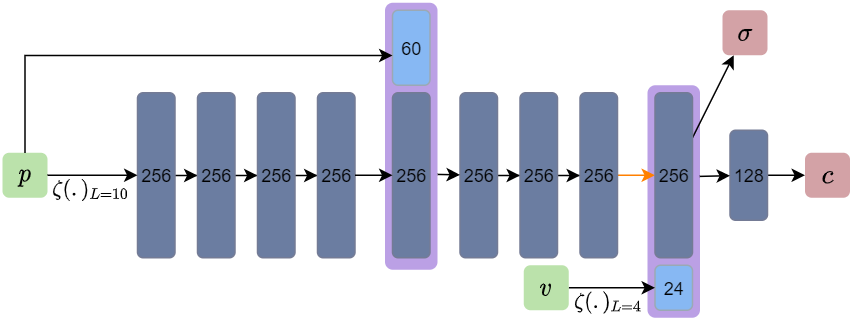
\includegraphics[width=0.9\textwidth]{figures/mlp_nerf.png}
    \caption{MLP used in NeRF \cite{mildenhall2020nerf} Dark blue boxes represent hidden layers. Black arrows indicate FC-layers with sigmoid activation, orange arrows - FC-layers without activation. Green boxes are inputs: $p$ is a 3D sample point, $v$ is a 3D vector of viewing direction. Red boxes are the outputs: $\sigma$ is 1D volume density, $c$ is a 3D color value. $\zeta(.)$ stands for positional encoding function that maps inputs into higher dimensional space $\mathbb{R}^{2L}$ (more in \Cref{subsec:pos_enc}}
    \label{fig:mlp_nerf}
\end{figure}

\cite{mildenhall2020nerf} propose to use a Multi-Layer Perceptron (MLP) as a representation
of an implicit function $F = F_\Theta$ with parameters $\Theta$.
The scheme structure of original NeRF's MLP is outlined in \Cref{fig:mlp_nerf}.
The position $p(z)$ is first encoded using position encoding function $\zeta(\cdot)$ (positional encoding is described in section \ref{subsec:pos_enc}) and then is processed with 8 fully-connected neural layers with ReLU activations.
The resulting feature vector is then concatenated with positionally encoded vector direction $v$
before the the volume density $\sigma(p(z))$ and the color value $c(p(z), v)$ is outputed.
The important concept here is that $\sigma$ only depends on point $p(z)$
whilst the color value $c$ is view dependant as well.
This setting is required to encourage the MLP to be multi-view consistent.

In order to perform the volume rendering, the continuous integral from equation \Cref{eq:rendering_equation} has to be solved.
One can estimate this integral using a discrete set of densely sampled points as proposed by \cite{mildenhall2020nerf}.
Separating each ray into $N$ bins and drawing random samples from each bin
makes the representation able to learn continuous function
while only using finite number of samples.
The estimate for the integral $C(p, v)$ will have a form (\cite{mildenhall2020nerf}, \cite{max1995optical}):

\begin{equation}
    \label{eq:integral_estimation}
    C(p, v) \approx \sum_{i=1}^{N} \tau_c(p_i) (1 - \exp (-\sigma(p_i) \delta_i)) c(p_i, v),
\end{equation}
where $p_i = p(z_i)$ for brevity, $\tau_c(p_i) = \exp (-\sum_{j=0}^i \sigma(p_j) \delta_j )$ is the accumulated transmittance and $\delta_i = z_{i+1} - z_i$ is the distance between adjacent sample points.

\subsection{Positional encoding}
\label{subsec:pos_enc}

Neural networks are known as a highly representative class of functions (\cite{hornik1989multilayer}).
However, recent works (\cite{rahaman2019spectral}, \cite{tancik2020fourfeat}) demonstrate the tendency of
biasing towards low frequency functions during training of deep neural networks.
The results can be smoothed and blurry as frequency-dependant learning speed
is much slower for high-frequency parts of the scene.
\cite{rahaman2019spectral} show that one can highly improve the quality of the MLP outputs
by using an embedding, which maps inputs to a higher dimensional space before passing them to the MLP.

The positional encoding function $\zeta(p) : \mathbb{R} \xrightarrow{} \mathbb{R}^{2L}$ as proposed by \cite{mildenhall2020nerf}, \cite{vaswani2017attention} is represented by Fourier series in the following form:

\begin{equation}
    \label{eq:positional_encoding}
    \zeta(p) = (\sin(2^0\pi p), \cos(2^0\pi p), ..., \sin(2^{L-1}\pi p), \cos(2^{L-1}\pi p))
\end{equation}


\subsection{Hierarchical sampling}
\label{subsec:hierarchy_sampling}

The proposed approach is ineffective in a way that it tends to generate a lot of unimportant samples
that lie on a free space and do not make contribute much.
To solve that authors propose the hierarchical volume sampling algorithm (similar to \cite{levoy1990efficient}),
when another "coarse" neural network is used in order to roughly estimate volume densities along the ray.
This insight is then used to perform a more informed sampling of main ("fine") network.
The "coarse" network is being optimized along with the main network, which can be considered as an overhead.
However, taking into account the increase of training convergence the overall training gets more efficient.


\subsection{Optimization}

The fully-differentiable formulation of the problem makes it possible
to optimize network parameters $\Theta$ without any 3D supervision.
This is done using the back-propagation approach from the differences
between rendered predictions and ground truth images.
This task therefore is reduced to the minimization problem of the loss function.
The original method by \cite{mildenhall2020nerf} for loss function uses the following formulation:
\begin{equation}
    \mathcal{L} = \sum_{(p_0, v) \in \mathcal{B}} \norm{ C_c(p, v) - C^*(p, v) }^2_2 + \norm{ C_f(p, v) - C^*(p, v) }^2_2,
\end{equation}
where $\mathcal{B}$ is the set of sampled rays in each batch,
$C^*$ is the target color value of the view ray $v$ and
$C_c(p, v)$, $C_f(p, v)$ - are the predicted colors for the view ray $v$ of the coarse and fine networks respectively.

Another regularization term can be added to this loss function as proposed by \cite{Lombardi_2019}.
The beta-distribution regularizer $\Omega(\cdot)$
forces the ray transmittance from the fine network $\tau_c$ to be close to $0$ or $1$:
\begin{equation}
    \Omega(\tau_c(p_i)) = \log(\tau_c(p_i)) + \log(1 - \tau_c(p_i))
\end{equation}
This helps the network to better handle background colors and get cleaner render after all.
This regularization term is used in NSVF work (\cite{liu2021neural})
that is described in \Cref{subsec:NSVF}
and NRF work (\cite{bi2020neural}) that is described in \Cref{subsec:NRF}



\subsection{Sparse Voxels Octree}
\label{subsec:NSVF}
The described approach is already able to represent scenes with high accuracy.
However, the very inefficient way of sampling points along rays
makes the training very slow and tough,
since the model has to be repeatedly evaluated on unimportant samples
of free space or occluded regions that do not make a worthwhile contribution to the finally rendered color value.
The \textit{hierarchical sampling} strategy alleviates the problem,
but does not solve it completely.
The method in its formulation therefore is still barely practical.


\cite{liu2021neural} propose another framework
that is able to increase the efficiency of this method
and make the training time by up to an order of magnitude faster.
The main contribution is the usage of sparse voxel octrees (\cite{laine2011EfficientSV}) to divide space into voxels
that are efficiently used for training MLPs with shared parameters.

This approach requires a slight elaboration on the problem formulation.
Let the whole scene being fully contained in a set of $K$ sparse voxels: $\mathbb{V} = \{V_k\}_{k=1}^K$.
The scene can then be represented as a set of voxel-bounded implicit functions
\begin{equation}
    F(p, v) = F_\Theta^i(g_i(p), \zeta(v)), \forall p \in V_i,
\end{equation}
where each function $F_\Theta^i$ is modelled with an MLP with shared parameters $\Theta$:
\begin{equation}
    F_\Theta^i: (g_i(p), \zeta(v)) \xrightarrow{} (c, \sigma), \forall p \in V_i
\end{equation}
Here $g_i(p)$ is the representation of $p$ that is defined as:
\begin{equation}
    g_i(p) = \zeta ( \chi ( \{\Tilde{g_i}(p_j^*)\}_{j=1}^8 ) ),
\end{equation}
where $\{p_j^*\}_{j=1}^8, p_j^* \in \mathbb{R}^3$ is the set of eight vertices of voxel $V_i$,
$\Tilde{g_i} \in \mathbb{R}^d$ represent the feature vectors that are stored for each vertex of voxel $V_i$,
$\chi(\cdot)$ stands for trilinear interpolation,
and $\zeta(\cdot)$ is a post-processing function,
which corresponds to positional encoding function explained in \ref{subsec:pos_enc}.


\begin{figure}[t]
    \label{fig:nsvf_structure}
    \centering
    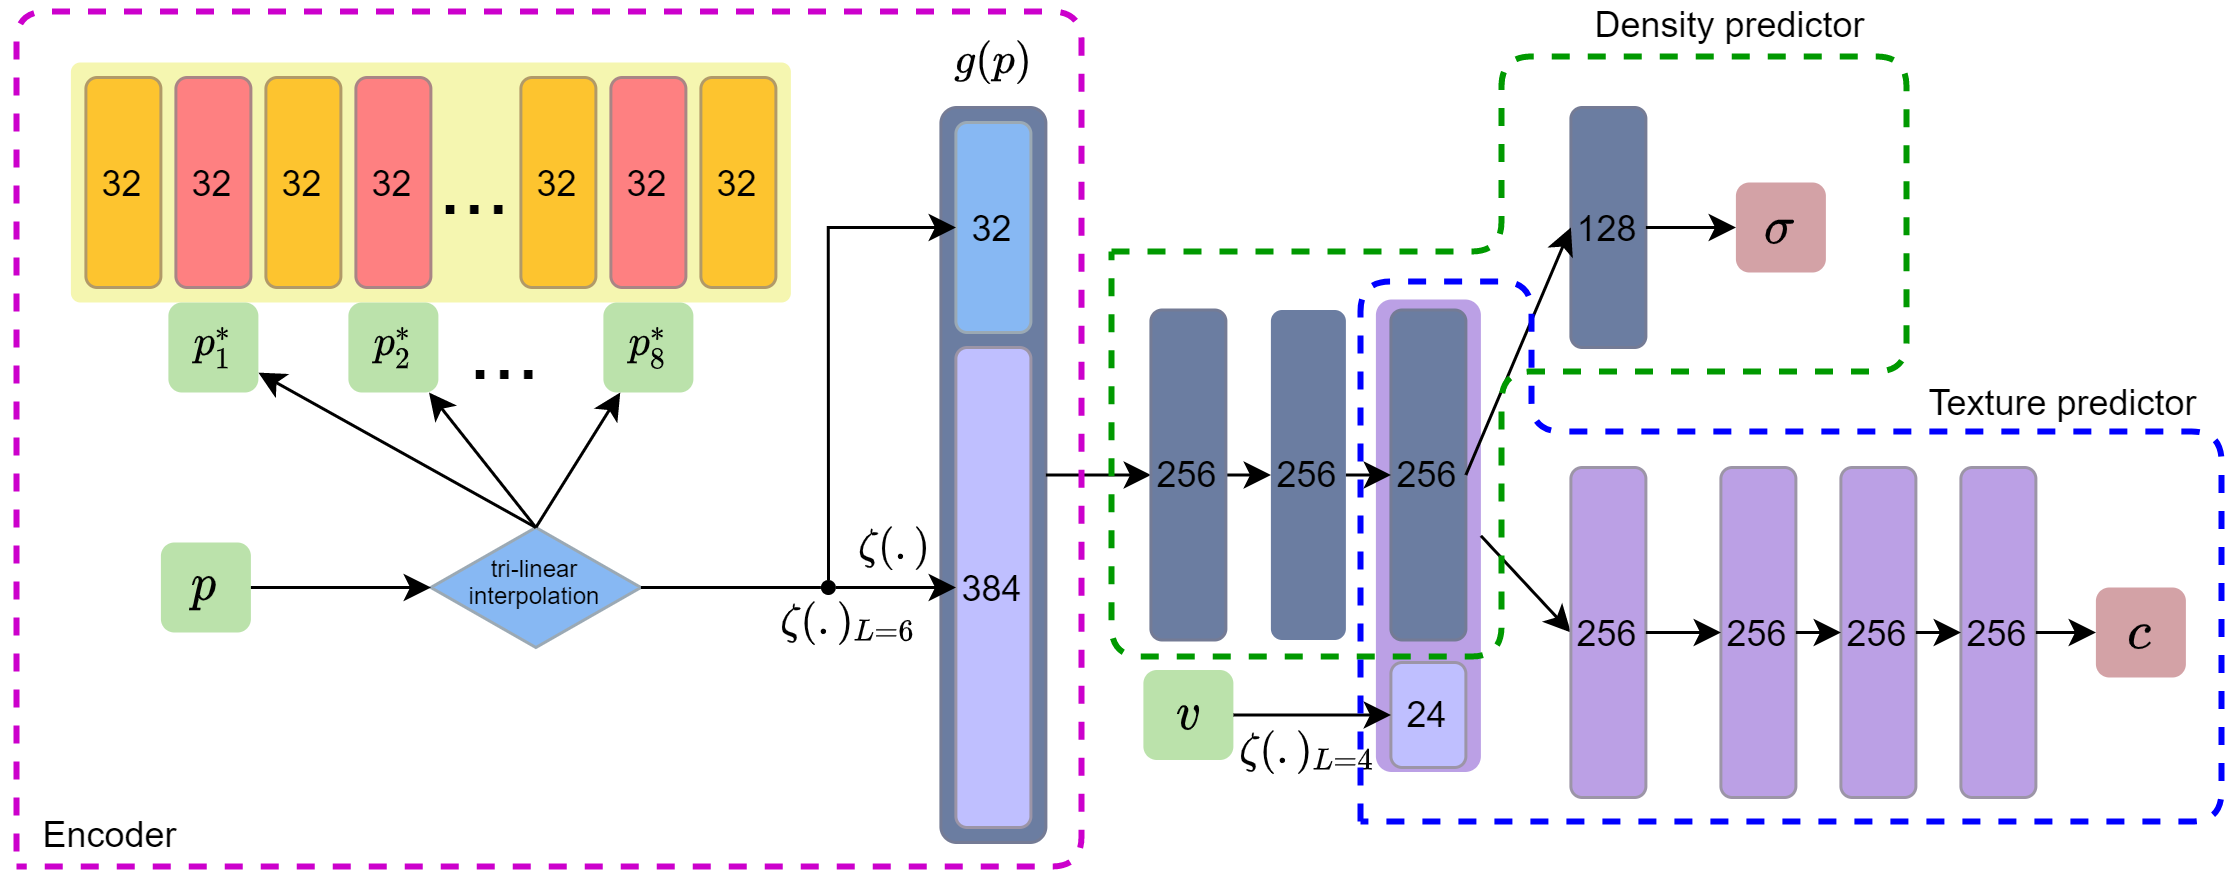
\includegraphics[width=0.9\textwidth]{figures/vanilla_nsvf.png}
    \caption{Network structure of the NSVF approach \cite{liu2021neural}.
Same notation as for \Cref{fig:mlp_nerf} is used.
Dotted lines denote semantic parts of the presented structure:
pink, green and blue dotted lines stand for encoder, density predictor and texture predictor respectively.
\textit{Trilinear interpolation} block denotes interpolation of the sample point $p$ between voxel embeddings.}
\end{figure}

The proposed network structure is outlined in \Cref{fig:nsvf_structure}.
The encoder part that is denoted with pink dotted line
consists of only one layer comparing to the original NRF network
where the encoder part consists of 5 deep layers.
The density predictor (green dotted line) remains the same.
The texture predictor (blue dotted line) is deeper comparing to the NeRF model.
The overall model structure is slightly shallower comparing to the original NeRF network,
which is still sufficient due to the distributed way of storing voxel embeddings in the voxel vertices.

The volumetric rendering itself does not undergo any significant changes
except for some additional steps that have to be performed.
The sampling of the ray is only performed on the intervals of intersection with voxels $V_i$.
This allows to reject a descent amount of unimportant samples.
A very efficient Axis Aligned Bounding Box (AABB) ray intersection algorithm (\cite{haines1989essential}) is applied here
to extract the above mentioned intervals.
Another step is \textit{early termination}, which reduces the number of samples that have to be processed.
Since solid surfaces does not imply color values being dispersed along the ray,
the sample points that are behind the surface would be needless.
The technique here is to straight forwardly stop evaluating points,
that have an accumulated transmittance lower than some threshold.

\subsection{Voxels pruning and refinement}
\label{subsec:pruning}

The training on the scene begins with the octree,
which consists of $N$ voxels that fit in bounding box of the whole scene
and cover all parts of the scene.
One can get rid of non-essential voxels by performing a \textit{self-pruning} procedure.
This technique leverages the property of neural radiance fields
to extract some coarse scene geometry during early training iterations.
The decision if voxel is going to be pruned is made by uniformly sampling $G$ points inside the voxel
and comparing the minimum transmittance value with some threshold value $\gamma$ or more formally when:
\begin{equation}
    \underset{j=1 \dots G}{min} {\exp (- \sigma (g_i(p_j)))} > \gamma, p_j \in V_i, V_i \in \mathbb{V},
\end{equation}
where $\sigma (g_i(p_j))$ is the model prediction for $\sigma$ when processing $g_i(p_j)$.
The pruning procedure has to be performed regularly as the accuracy of the model increases as it gets more and more trained,
which means that more voxels can be pruned and therefore rejected from processing.

As model learns more detailed representation of the scene it becomes necessary to refine voxel structure.
During the refinement procedure each voxel is being subdivided into $2^3$ subvoxels by halving the voxel size.
Ray sampling steps are also being halved at this point in order to correspond new voxel size value.
The feature representation vectors $\Tilde{g_i}$ of the new vertices are initialized similarly to calculating $G_i(p)$,
namely using trilinear interpolation function $\chi(\cdot)$.
This scheme allows to achieve more detailed scene representation
and also increases the model capacity.



\subsection{Neural Reflectance Fields}
\label{subsec:NRF}

Although the neural radiance fields approach is able to produce realistic renderings under novel view conditions,
one of main limitations of this method is the inability to handle any kind of visual effects related to dynamic light conditions.
The core assumption of these approaches is a static illumination,
which is implicitly presented in the color values of the rendered images.
This in turn does not allow to change illumination on the rendering phase.

\cite{bi2020neural} propose the framework for eliminating this exact limitation.
Authors introduce neural reflectance field (NRF), which is the neural scene representation
that in addition to scene geometry also encodes normal and reflectance properties of the scene.
This approach allows to evaluate an explicit reflectance model at the selected point after all.
Although \cite{bi2020neural} focus on the microfacet bidirectional reflectance distribution function (BRDF) (\cite{walter2007microfacet}),
any other reflectance model can be used within this method as well
(i.e. authors also show some results of furry objects using hair reflectance model \cite{kajiya1989fur}).

This method uses the same rendering framework as proposed by \cite{mildenhall2020nerf}.
Assuming that the volume containing the scene to be only scattering volume (i.e. there are no emission or absorption processes),
the corresponding rendering equation \Cref{eq:rendering_equation} (\cite{Novak18volumeSTAR}) looks similarly
except for operating with radiance values $L$ instead of color values $c$:
\begin{equation}
    L(p, v) = \int_0^\infty \omega(p(z)) \cdot L_s(p(z), v) dz = \int_0^\infty \tau_c(p(z)) \sigma(p(z)) \cdot L_s(p(z), v)dz,
\end{equation}
where $L_s(p(z), v)$ denotes the scattered light at point $p(z)$ along direction $v$.

In general case $L_s$ is calculated by integrating incident radiance along the whole unit sphere $\mathbb{S}$:
\begin{equation}
    \label{eq:radiance_Li}
    L_s(p, v) = \int_\mathbb{S} f_p(p, v, l) L_i(p, l)dl,
\end{equation}
where $l$ is the 3D Cartesian representation of directions of the incident radiance $L_i(p, l)$.
$f_p(p, v, l)$ is the phase function, which controls
how the light that comes from $l$ scatters at point $p$ if viewing from $v$.

\cite{bi2020neural} only assume single light source setting
and the reflectance function as the phase function,
which allows to simplify \Cref{eq:radiance_Li}:
\begin{equation}
    L_s(p, v) = f_r(p, v, l, n(p), R(p)) L_i(p, l),
\end{equation}
where $f_r$ denotes a differentiable reflectance function
with parameters $R$.
Normal vector $n$ is also required for evaluation of reflectance model $f_r$.
$L_i(p, l)$ is the radiance that arrives from direction $l$ and can be calculated using light intensity $L_l(p)$
and the transmittance value $\tau_l(p, l)$,
which indicates the loss of light from the light source to the sample point $p$ along light ray $l$, as follows:
$L_i(p, l) = \tau_l(p, l) L_l(p, l)$.
The light attenuation coefficient $f_{att} = \frac{1}{k_c + k_l d + k_q d^2}$ \im{???citation to blog page???} is considered inside the $L_l$ term:
$L_l(p, l) = f_{att} \cdot I$,
where $k_c$, $k_l$ and $k_q$ are attenuation factors,
$I$ is the point light intensity.
% where $d$ is distance from sample point $p$ to the light source
% and $r$ is the light's radius (assuming light source to be an emissive sphere with radius $r$) and 
In my experiments the attenuation coefficients $k_c = k_l = 0$ and $k_q = 1$ were used,
so the attenuation coefficient is inverse proportional to squared distance between light sample point and light source:
$f_{att} = \frac{1}{d^2}$

Combining these equations together and applying the same technique for numerical integral estimation
as used by \cite{mildenhall2020nerf} and \cite{liu2021neural} gives the following formulation of \Cref{eq:integral_estimation} for NRF:
\begin{equation}
    \label{eq:integral_estimation_nrf}
    L(p, v, l) \approx \sum_{i=1}^N \tau_l(p_i, l) L_l(p_i, l) f_r(p_i, v, l, n(p_i), R(p_i)) \tau_c(p_i) (1 - \exp (-\sigma(p_i)\delta_i))
\end{equation}
Here $\tau_l$ plays the same role for light ray $l$
as $\tau_c$ operates for view ray $v$.
It is evaluated similarly along the light ray $l$:
$\tau_l(p'_i, l) = \exp (-\sum_{j=1}^M \sigma(p'_j) \delta'_j)$,
where $p'(z') = p'_0 + z' \cdot l$ are sample points that are additionaly sampled along the light ray $l$ and $\delta'_j = z'_{j=1} - z'_j$.


\begin{figure}[t]
    \centering
    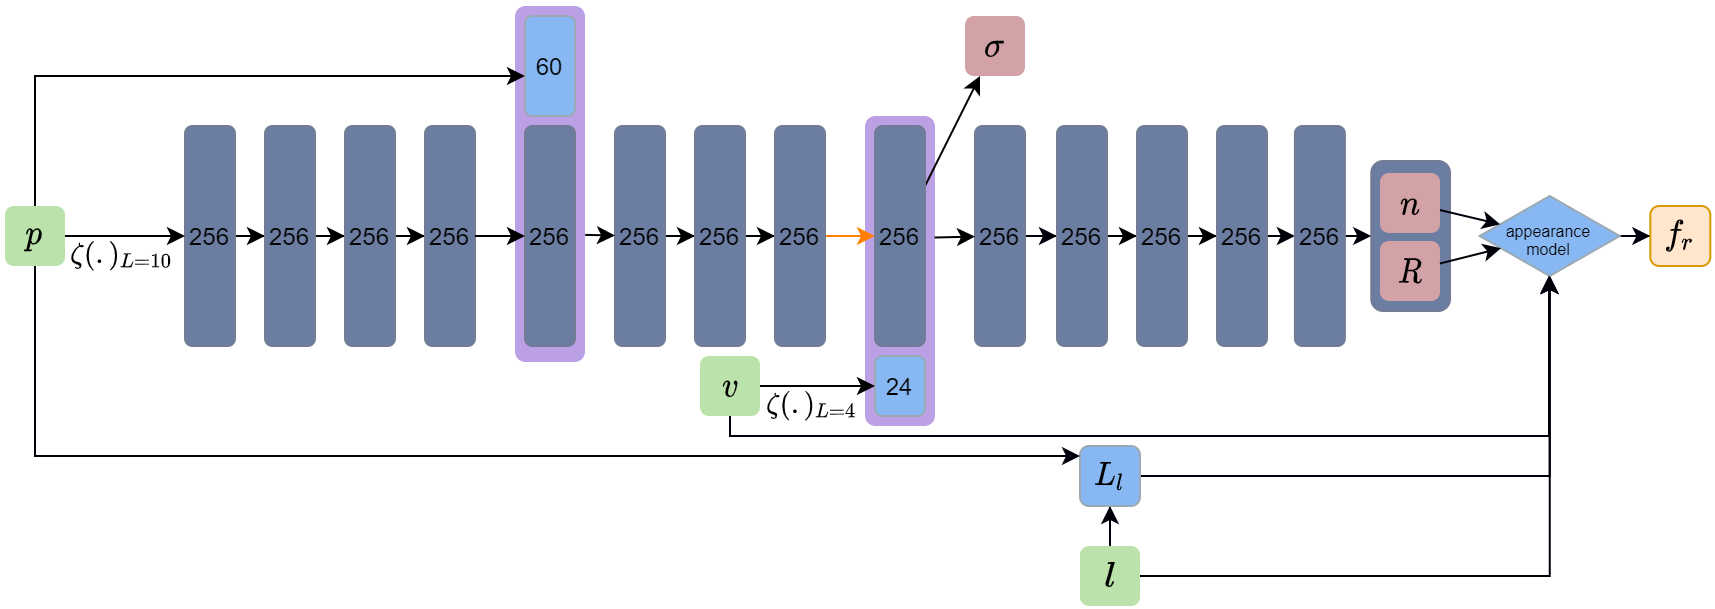
\includegraphics[width=0.9\textwidth]{figures/vanilla_nrf.png}
    \caption{MLP structure of the NRF \cite{bi2020neural} approach.
The overall network structure echoes the original NeRF model.
14 deep layers are used (instead of 10 in NeRF).
The appearance model block represents BRDF $f_r$
that is evaluated for each sample point $p$.
To this end network outputs normal $n \in \mathbb{R}^3$
and BRDF parameters $R \in \mathbb{R}^m$ ($m=4$ for microfacet BRDF).
$L_l$ denotes light intensity with consideration to distance attenuation.
}
    \label{fig:nrf_structure}
\end{figure}

The architecture of the MLP is outlined in \Cref{fig:nrf_structure}.
The deeper structure is used as the model capacity has to be increased
due to higher complexity of the task.
For each view sample point $p$ model outputs both normal vector $n$ and parameters $R$,
which are requires by the selected BRDF model.
For the microfacet BRDF (\cite{walter2007microfacet}) $R$ consists of 3-dimensional albedo value
and 1-dimensional roughness value.



This formulation covers the general case when light source can be located at arbitrary position ('arbitrary setting').
Since the $l$ and $v$ vectors are different,
the additional sampling of light ray for each view sample point is required.
It makes this problem infeasible.
However, \cite{bi2020neural} show that one specific light setting exist,
which can be used to handle this problem.
When the light ray $l$ coincide with the view ray $v$,
then sampling points $p(z)$ and $p'(z)$ would be the same,
which in turn means that $\tau_c(p_i) = \tau_l(p_i)$ ('co-located setting').
In this case there is no need in additionally sampling light rays,
which leave the processing time requirements on the same level as original work by \cite{mildenhall2020nerf}.
% \Cref{fig:colocated_light_source} \im{add figure} shows this process in more details.
Another advantage of this setting is that it has an accessible real-world analogy.
In particular, all of modern cellphones are equipped with cameras
and flash lights that are placed close to each other.
On the scale of the scene this displacement can be neglected and the setting can be considered to be co-located.

The co-located setting results in a very sparse sampling of the scene in terms of light-view directions.
During training there basically are no other samples than those
where angle between light and view rays is greater than zero.
This fact negatively affects the overall training performance,
although \cite{bi2020neural} proves that even with these restrictions
the network is still able to generalize and reconstruct the scene appearance in high quality.
Authors also show some renders where the 'arbitrary setting' had been used during prediction phase.





\section{Explicit Neural Reflectance Field}
\label{sec:explicit_scheme}

The described above methods have already achieved some appealing results.
However, all of them have their own limitations that in either event reduce the performance either qualitatively or quantitatively.

Since the NRF approach \cite{bi2020neural} is based on NeRF, it inherits its poor performance behaviour
and forces it to be only applicable for the 'co-located setting'.
Although the authors are even able to render the scene within 'arbitrary setting'
when only being trained on the co-located dataset,
the sparsity of the training dataset is still highly affects network's generalization opportunities.

\cite{liu2021neural} in turn propose the technique for increasing the training time and effectiveness of the training
for the color-based original NeRF approach.
The usage of gradually refined octrees gives more control over the sampling process
and makes the whole training phase faster.

\begin{figure}[t]
    \centering
    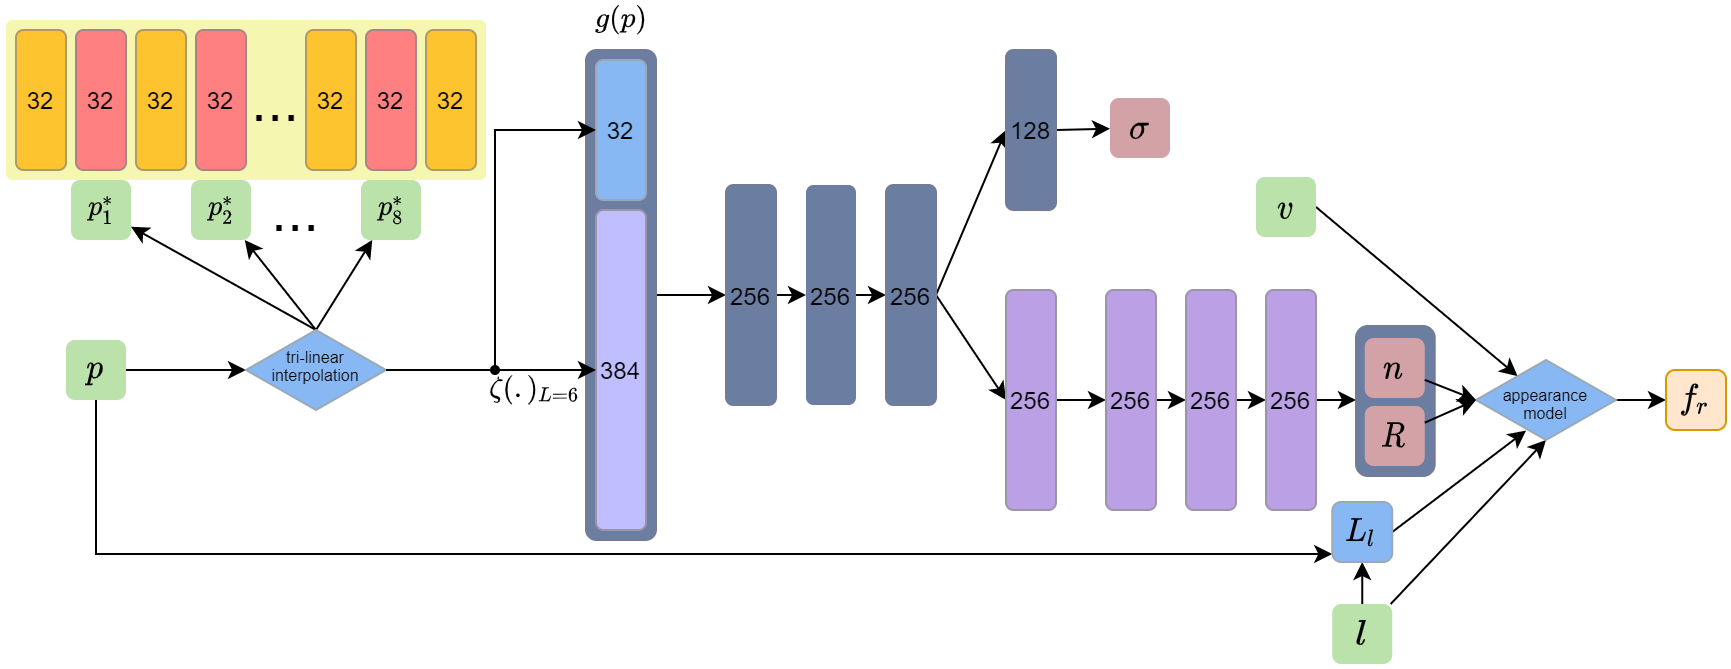
\includegraphics[width=0.9\textwidth]{figures/explicit_scheme.png}
    \caption{Model architecture for the 'explicit scheme'
    (\Cref{sec:explicit_scheme}).
The overall structure follows one from NSVF work.
The outputs of the network are similar to the NRF model.
BRDF evaluation ('appearance model' block) is required for achieving $f_r$ value.
    }
    \label{fig:mlnrf_bfex}
\end{figure}

Since both works NSVF and NRF use original NeRF framework,
in particular similar numerical integral estimation,
the process of reformulating NSVF problem to work with light radiances instead of color values is fairly straight forward.
For the integral estimation \Cref{eq:integral_estimation} is directly replaced with \Cref{eq:integral_estimation_nrf}.
The network architecture follows the guidelines from the NSVF work,
namely the encoder is shallow while texture predictor is deeper
comparing to the original NeRF method.
Appearance model block (right blue rhombus) includes BRDF evaluation,
which results in $f_r$ value required for final radiance calculation (using integral estimation formula \cref{eq:integral_estimation_nrf})

In order to train model on arbitrary light dataset
an additional step of light rays sampling and volume density prediction is needed.
This requires some nested model evaluations in order to retrieve $\sigma$ values at light sample points.
This is a quite memory intense part, however the lower model size comparing to the NRF approach makes it more accessible.
Another key note here is that there is no need in getting texture field predictions,
as for light rays the only valuable information is the volume density.
This allows to only evaluate the corresponding part of model.

Another key point here is the format of the dataset.
The NeRF and NSVF methods only work with color values,
which allows them to use the LDR images in the datasets
(i.e. PNG, JPG image formats and others).
However, NRF approach imply light intensity values that are integrated in final radiance calculations.
The LDR images are usually lacking the information of radiances
and only operate with color values.
All these facts make the LDR images bad candidates for the training dataset.
One should instead consider using HDR images (i.e. HDR, EXR formats).

The point light intensity value $I$ that takes part in calculation of $L_l(p, l) = f_{att} \cdot I$
represents the radiation power of the light source.
This value is known when processing artificially generated scenes
and thus can directly be used as value of $I$.
The real-world scenes (e.g. captured with the cellphone and flash light)
on the contrary does not have the exact light intensity value.
One could estimate the power of the flash light, but this would give only a rough estimation.
To make the method robust to this kind of estimations,
the light intensity value $I$ is passed to optimizer (along with other model parameter $\Theta$).
This technique requires some robust estimation of $I$ as an initialization value as well as an increased learning rate.



\section{In-Voxel Light Approximation}

Using sparse octree voxels for increasing the efficiency of the method
makes the whole problem feasible within some commonly accessible hardware.
However, the training procedure still remained highly computationally expensive and memory demanding
and therefore very slow in training or still even intractable for high resolution scenes.

The main load of this approach still remains in the additional sampling of light rays
and the consecutive model evaluation for calculating $\tau_l(p', l)$.
This fact leads to the task of minimizing the overhead that is caused by calculating light ray transmittances.

Predictions of volume densities at view ray sample points have primary importance
as they contribute into the final radiance value the most.
This assumption brings to the fact that light rays are not required
to be sampled as densely as view rays to remain the same level of accuracy.
Thus the lower number of points can be sampled on the light rays,
which would result in lower memory and time consumption.
However, this approach only alleviates the problem while not solving its route cause.

The octree structure that is used to encode feature vectors $\Tilde{g_i}$ in the corners of voxels
represent itself a coarse geometry of the scene.
Starting with only a few voxels that cover the whole bounding box around the scene,
the voxels undergo the \textit{self-pruning} and \textit{refinement} procedure (explained in \Cref{subsec:pruning}),
which increase the detailing capabilities of the octree
by increasing the number of voxels, lowering its sizes and rejecting empty voxels.
After only a few steps of the aforementioned operations the overall voxel structure
repeats scene geometry with a considerable amount of accuracy.
These voxels that intersect with the light rays can be used as an estimation of volume densities.

% \begin{figure}
%     \begin{tabular}{ccc}
%           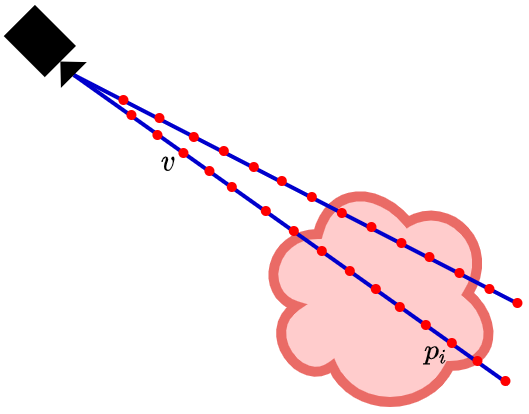
\includegraphics[width=0.1\textwidth]{figures/sampling_nerf.png}
%           & 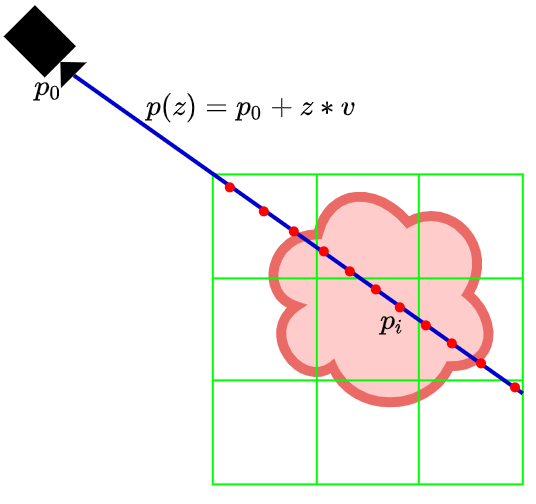
\includegraphics[width=0.1\textwidth]{figures/sampling_nsvf.png}
%           & 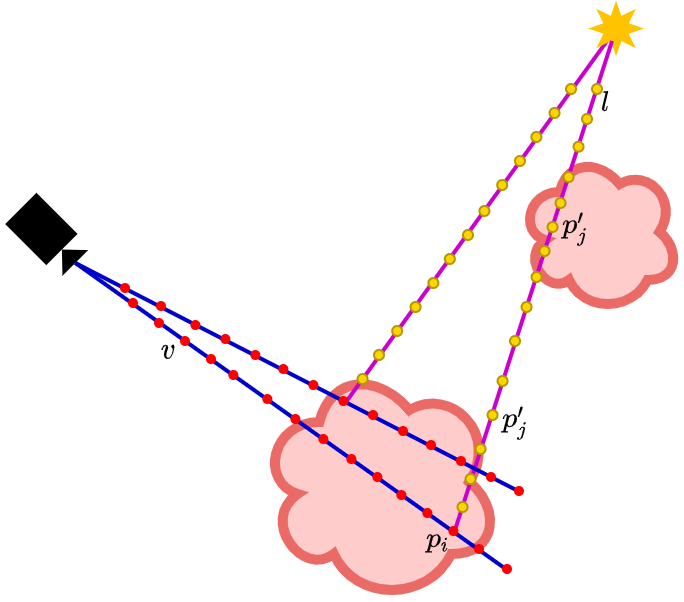
\includegraphics[width=0.1\textwidth]{figures/sampling_nrf.png}
%           \\(a) NeRF \cite{mildenhall2020nerf} & (b) NSVF \cite{liu2021neural} & (c) NRF \cite{bi2020neural}
%           \\[6pt]\multicolumn{3}{1}{
%               \begin{tabular}{cc}
%                 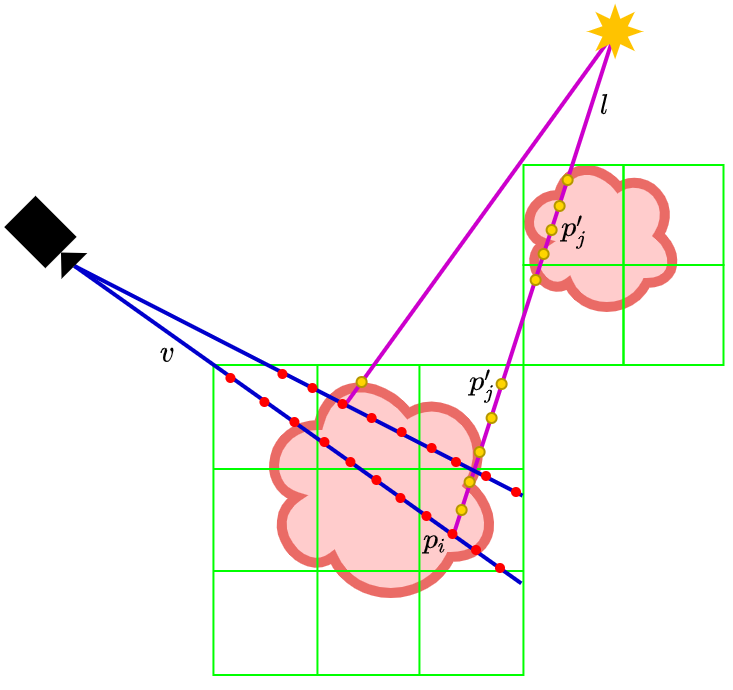
\includegraphics[width=0.1\textwidth]{figures/sampling_bfex.png}
%                 & 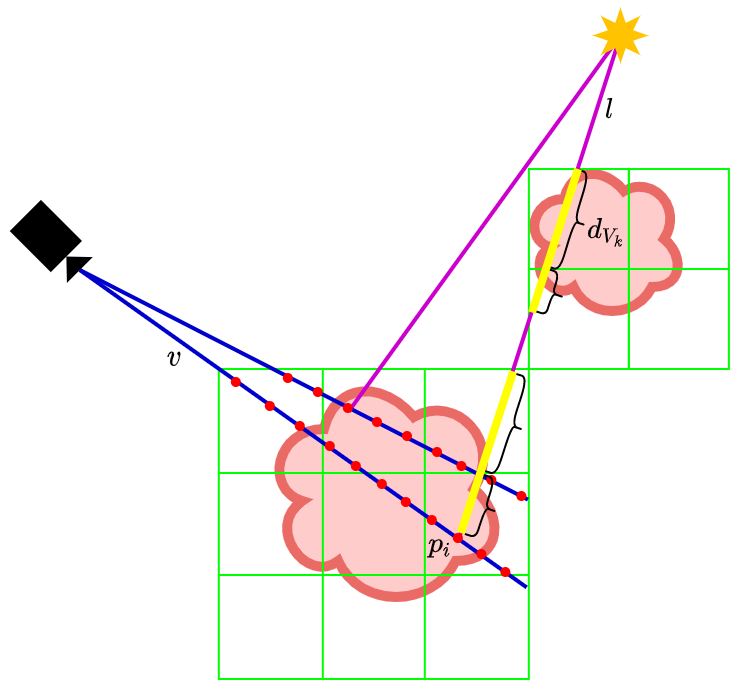
\includegraphics[width=0.1\textwidth]{figures/sampling_iva.png}
%                 \\[6pt](d) 'Brute-force' & (e) In-voxel approximation
%               \end{tabular}
%           }
%     \end{tabular}
%     \caption{caption}
% \end{figure}
\begin{figure}
    \begin{tabular}{ccc}
          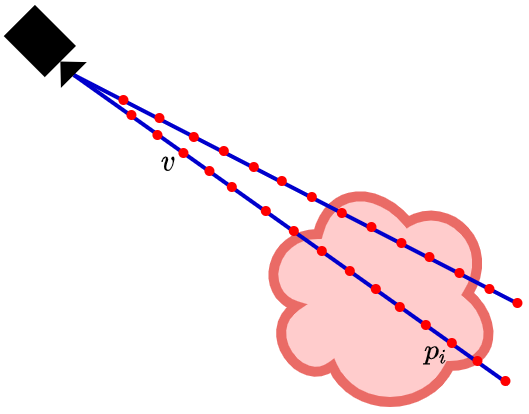
\includegraphics[width=0.285\textwidth]{figures/sampling_nerf.png}
          & 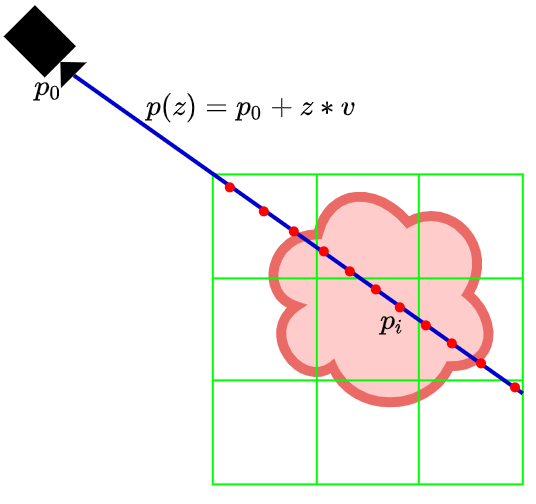
\includegraphics[width=0.26\textwidth]{figures/sampling_nsvf.png}
          & 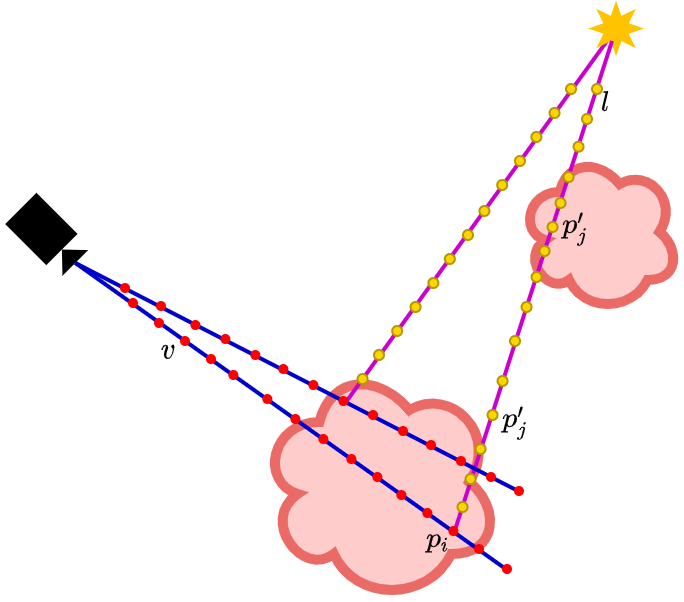
\includegraphics[width=0.355\textwidth]{figures/sampling_nrf.png}
          \\(a) NeRF \cite{mildenhall2020nerf} & (b) NSVF \cite{liu2021neural} & (c) NRF \cite{bi2020neural} (general)
          \\[6pt]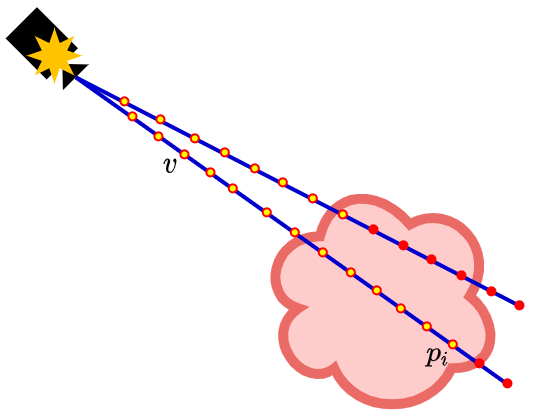
\includegraphics[width=0.26\textwidth]{figures/sampling_nrf_colocated.png}
          & 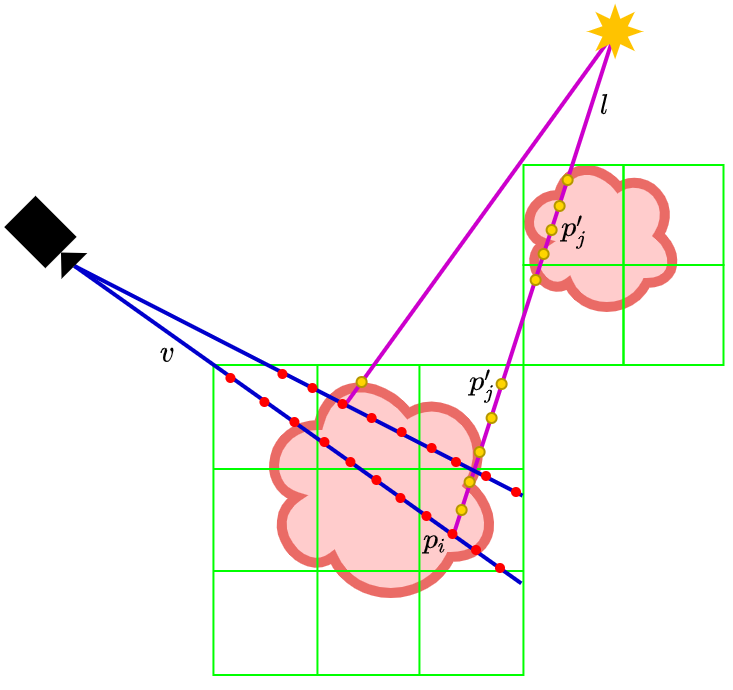
\includegraphics[width=0.32\textwidth]{figures/sampling_bfex.png}
          & 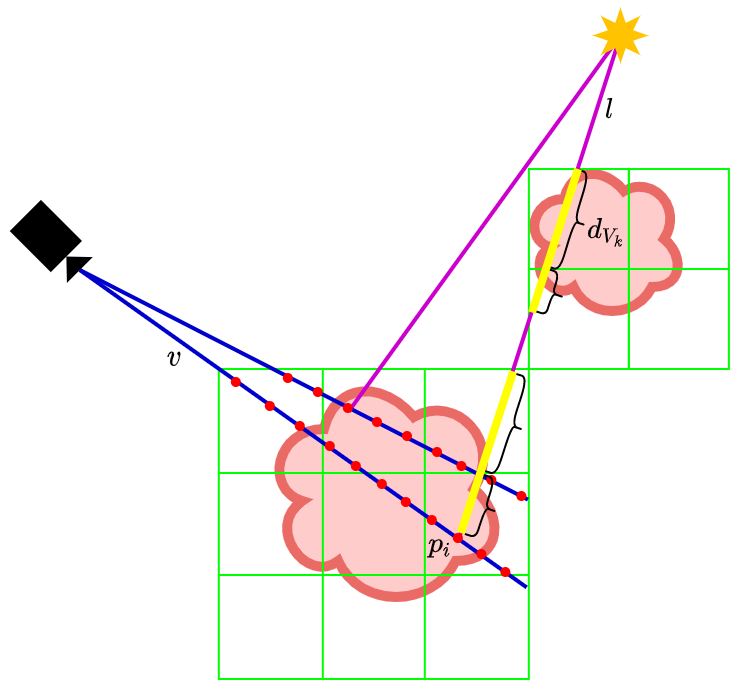
\includegraphics[width=0.32\textwidth]{figures/sampling_iva.png}
          \\(d) NRF (colocated) & (e) 'Brute force'& (f) In-voxel approximation
    \end{tabular}
    \caption{
Sampling techniques used in different approaches.
The 2D sketch schemes are used instead of 3D visualizations for simplicity.
Blue lines represent view rays $p(z)$ with direction vector $v$,
purple lines stand for light rays $p'(z)$ with light direction vector $l$
(only two of those are shown for brevity).
Right dots represent sampled view points $p_i$, yellow dots stand for light sample points $p'_i$.
Scheme (a) shows the original NeRF sampling technique without \textit{hierarchy sampling} (\Cref{subsec:hierarchy_sampling}).
Scheme (b) correspond to the NSVF sampling technique
that only occurs inside intersected voxels (represented by green boxes).
Scheme (c) shows sampling of the general case of the NRF approach
when light source is placed at arbitrary position.
Scheme (d) displays the 'colocated setting'
when point light source is positioned at the same location as camera.
In this case light sample points (yellow dots) coincide with the view sample points (red dots).
Scheme (e) correspond to the proposed in this work 'brute-force' approach
when light rays sampling is reduced by using the same voxel structure as in NSVF (fig. (b)).
Scheme (f) shows sampling in proposed in this work in-voxel approximation scheme.
View rays are sampled in a similar way as in NSVF approach
while light ray transmittances are estimated using travelled distances $d_{V_i}$
of the light ray inside voxels.
}
\label{fig:samplings}
\end{figure}

There are plenty of techniques that can be applied here in order to calculate light transmittances more efficiently.
The main proposed technique imply the assumption
that the volume density is homogeneously distributed inside the voxel.
This assumption is certainly wrong for general case,
but should give a fair estimation for the light ray transmittances.
In this case the travelled distance $d_{V_k}$ of the ray inside voxel $V_k$
can be used to weigh some value $\hat{\sigma_{V_k}}$ (\Cref{fig:samplings} f):
\begin{equation}
    \tau_l(p_i, l) = \exp \sum_{V_k \in \mathbb{V}^*} -\hat{\sigma}_{V_k} \cdot d_{V_k},
\end{equation}
where $\tau_l(p_i, l)$ is the light transmittance value at the view sample point $p_i$
and $\mathbb{V}^* \subset \mathbb{V}$ is the set of voxels $V_k$
that have been intersected by the light ray $p'(z') = p'_0 + z' \cdot l$.

The model can be periodically evaluated to predict the values of $\hat{\sigma}_{V_k}$ and consequently calculate $\tau_l$.
The period of evaluation can be similar to periods for \textit{self-pruning} and \textit{refinement} procedures
as some coarse value would already give an acceptable level of certainty.

Some other options can be applied here such as:
\begin{enumerate}
    \item calculate $\hat{\sigma}_{V_k}$ using points sampled in centers of voxels $V_k \in \mathbb{V}^*$
    \item calculate mean $\hat{\sigma}_{V_k}$ value from points of intersection of light ray with voxels $V_k \in \mathbb{V}^*$
    \item assign $\hat{\sigma}_{V_k} = \const, \forall V_k \in \mathbb{V}^*$
\end{enumerate}



\section{Implicit Neural Reflectance Field}

The aforementioned methods that are proposed within this work
extend existing approaches in terms of efficiency for the problem of reproducing the scene under novel view and light conditions.
The novel light conditions is the essential requirement here
as it expects the method to not only account for color values
but also care about the reflectance of the surface.
Although, the NRF approach is formulated in general form
when any differentiable appearance model can be used for final radiance evaluation,
the result is still limited by the chosen BRDF.

\begin{figure}[t]
    \centering
    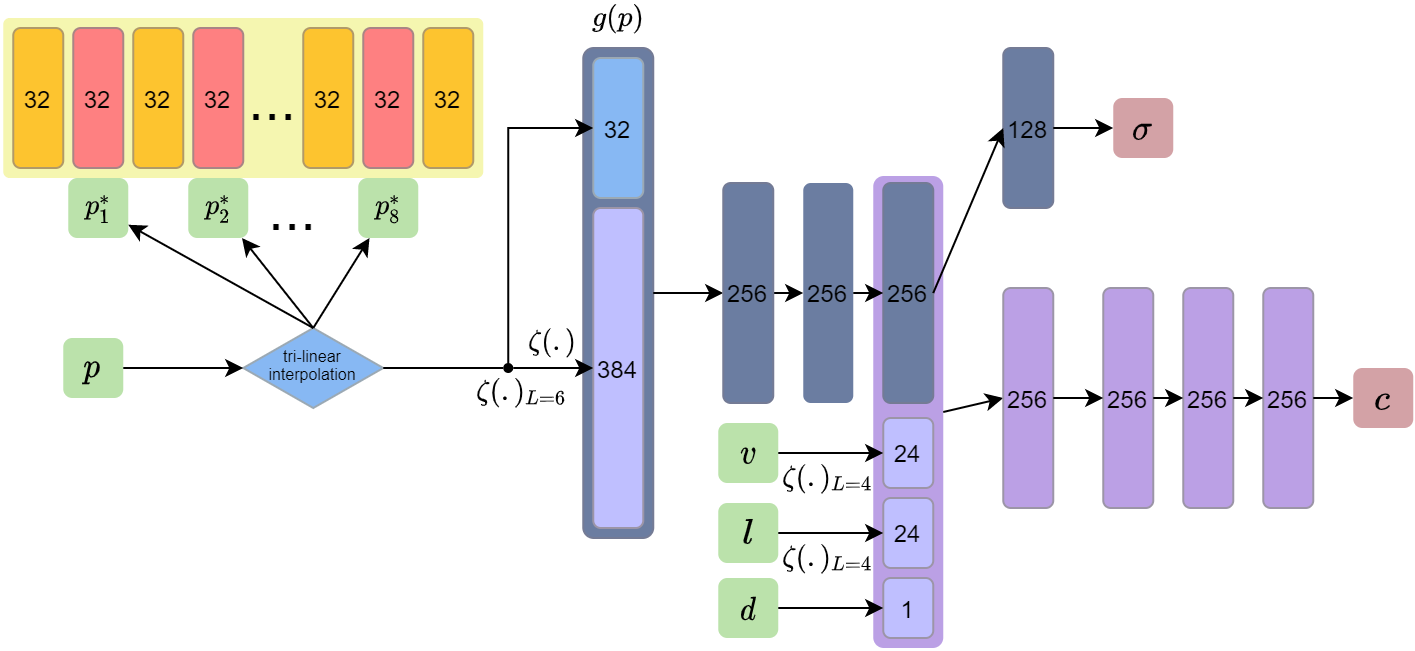
\includegraphics[width=0.9\textwidth]{figures/implicit_scheme.png}
    \caption{Network architecture for the implicit scheme.
The structure of the network mostly remains the same as in original NSVF work.
Some additional parameters such as light ray direction $l$
and distance $d$ from view sample point $p$ to the point light
are provided in advance into texture predictor.
}
    \label{fig:implicit_scheme}
\end{figure}

To expand these limitations one can shift the appearance evaluation burden to the deep neural network,
which is able to get trained for a very complex appearance representations.
This 'implicit scheme' would have a simpler neural network structure,
which is shown on \Cref{fig:implicit_scheme}.
The light interaction is performed here implicitly by providing 
the network the light direction $l$ as well as distance from sample point to the light source $d_i = \norm{p^l_k - p_i}$
as denoted on figure.
Light ray direction $l$ is also positionally encoded with the same $L$ as view ray direction $v$ is.

Another property of this technique will be the increased complexity of the learning function,
which would expect the network structure with greater capacity.

\im{\textit{Disadvantage: almost no control over implicit representation}}



% \section{Implicit Neural Reflectance Field}

% Existing BRDF models limits the type of scenes that can be captured
% and successfully reconstructed afterwards.
% To model object appearance one can employ neural network, which is able to get trained for a very complex appearance representations.
% In this work I \im{we?} call this technique as "Implicit scheme".

% Texture predictor not only is dependant on view direction,
% but also requires the light direction and distance to light source
% (for modelling the light attenuation effect).
% Figure \# shows the network structure for this approach.

% \begin{enumerate}
%     \item Light rays are not sampled (-> varying light transmittance either not considered or assumed to get learned by network\im{???})
%     \item |--> Tangential space for coordinates (and parametrization as half-vectors. not done)
% \end{enumerate}

% Since the appearance effects happen mostly in a local coordinate frame, the usage of the global direction vectors implies on the model to learn global to local coordinate system transformation. Although this is generally achievable, the overall complexity of the task can be too overwhelming for the model and some kind of correlations might affect the model. In order to increase the training performance this transformation can be done deterministically and the view and light directions in local coordinate frame are to be passed to the input of the model.

% The usage of the cartesian vectors is not very effective for reflectance representations. The half diff vectors (rusinkiewicz parametrization) can be used instead of positionally encoded l and v.
% \sm{or in combination with positional encoding}

% \section{In-Voxel Approximation}

% Using the octree allows to approximate light rays sampling inside voxels in order to increase the performance of the method.

% Instead of performing inverse CDF sampling as it is done for view rays, one can do the following:
% \begin{enumerate}
%     \item Bravely \sm{colloquial} assume the media homogenious inside voxels and boldly approximate it as constant
%     \item Under the same brave assumption perform some sampling inside the voxel once at N iterations (e.g. right after pruning has been performed)
%     \item The in-voxel sampling can be lighter than inverse CDF (e.g. just sample the center of voxel, or voxel corners + trilinear interpolation)
% \end{enumerate}







% NSVF proposed a good technique of using Sparse Voxel Trees in order to increase the rendering speed. However, the scene is still lacking the light interaction.

% One can achieve this by also passing light directions along with distance to the light source into the network, in order to make it distinguish different surface properties for different view and light directions.








% This is some test area for new mathematical helper macros to nicely visualize mathematical formulas.

% \section{Numbers}
% \begin{align}
%     \mathbb{C}
%     \qquad
%     \mathbb{R}
%     \qquad
%     \mathbb{Q}
%     \qquad
%     \mathbb{Z}
%     \qquad
%     \mathbb{N}
% \end{align}

% \section{Numbers with physical units}
% \begin{align}
%     \SI{1.23}{\meter\per\second}
% \end{align}
% \begin{align}
%     \si{\meter\per\second}
% \end{align}
% \begin{align}
%     \SI{1.23\pm0.45}{\meter\per\second}
% \end{align}
% \begin{align}
%     \SI{3e8}{\meter\per\second}
% \end{align}
% \begin{align}
%     \SI{32}{\giga\byte} = \SI{32e9}{\byte}
% \end{align}
% \begin{align}
%     \SI{32}{\gibi\byte} = \SI[exponent-base=2]{32e30}{\byte}
% \end{align}

% \section{Norm, Dot, Abs, Interval}
% \begin{align}
%     \pi = \const
% \end{align}
% \begin{align}
%     1 \in \interval{0}{2}
% \end{align}
% \begin{align}
%     1 \in \order{n}
% \end{align}
% \begin{align}
%     \evalat{ \frac{\partial f}{\partial x} }{ x = 0 }
% \end{align}
% \begin{align}
%     \norm{p} \qquad \norm{\frac{p}{2}}
% \end{align}
% \begin{align}
%     \abs{p} \qquad \abs{\frac{p}{2}}
% \end{align}
% \begin{align}
%     \dotproduct{p}{q} \qquad \dotproduct{\frac{p}{2}}{q}
% \end{align}
% \begin{align}
%     \crossproduct{p}{q} \qquad \crossproduct{\frac{p}{2}}{q}
% \end{align}

% \section{Vector, Matrix}
% \begin{align}
%     \vec{p} \qquad \vecarrow{p}
% \end{align}
% \begin{align}
%     \vec{p}^{\transposed}
% \end{align}
% \begin{align}
%     \gradient{\vec{p}}
% \end{align}
% \begin{align}
%     \divergence{\mat{A}}
% \end{align}
% \begin{align}
%     \laplacian{\mat{A}}
% \end{align}
% \begin{align}
%     \mat{A}
% \end{align}
% \begin{align}
%     \set{K} , K
%     \qquad
%     \set{N} , N
% \end{align}
% \begin{align}
%     \neighborhood{\vec{p}} = \left\{ \vec{q} \mid \norm{\vec{p} - \vec{q}} < \epsilon \right\}
% \end{align}

% \section{Set operations}
% \begin{align}
%     A \intersect B
% \end{align}
% \begin{align}
%     A \union B
% \end{align}
% \begin{align}
%     A \difference B
% \end{align}

% \section{Derivative, Integral, Sum, Probability}
% \begin{align}
%     \int_H x \, dx
% \end{align}
% \begin{align}
%     \sum_H x
% \end{align}
% \begin{align}
%     \probability{x}
% \end{align}
% \begin{align}
%     \probabilitygiven{x}{y}
% \end{align}
% \begin{align}
%     \expectation{x}
% \end{align}
% \begin{align}
%     \deviation{x}
% \end{align}
% \begin{align}
%     \variance{x}
% \end{align}


% \section{Lemma, Theorem, Corollary}
% \begin{lemma}
%     This is a lemma.
% \end{lemma}
% \begin{proof}
%     Proof of lemma.
% \end{proof}

% \begin{theorem}
%     This is a theorem.
% \end{theorem}
% \begin{proof}
%     Proof of theorem.
% \end{proof}

% \begin{corollary}
%     This is a corollary.
% \end{corollary}
% \begin{proof}
%     Proof of corollary.
% \end{proof}


 % Proposed method/solution

    % % % % % % % % % % % % % % % % % % % % % % % % % % % % % % % % % % % % % % % % % % % % % % % % % % % % % % % % % % % % % % % %

    
\chapter{Evaluation \im{(or Results?)}}
\label{chap:evaluation}

This chapter addresses results of the experiments and comparisons to other methods.


\section{Implementation details}

\begin{enumerate}
    \item Datasets
    \begin{enumerate}
        \item Synthetic datasets:
        \begin{enumerate}
            \item static/co-located/arbitrary
            \item Blender + python
            \item Blender point light intensity for light attenuation
        \end{enumerate}
        \item Real-world datasets: flower??? tac7
    \end{enumerate}
    \item Loss function: color + beta-regularizer
    \item Parameters: optimizer, lr, batch, coefficients
    \item Software/Hardware setup
    \item Time estimates
\end{enumerate}



% \section{Blender-Radiance coefficient}

% The light attenuation factor has to be taken into account in the explicit scheme.

% $L_o(x, \Omega_o) = L_e(x, \Omega_o) + \int_{H_i}{f_{BRDF}(\Omega_i, x, \Omega_o) L_i(x, \Omega_i) cos \Theta_i d\omega_i}$

% $L_i = \tau_l L_l$

% $L_l = f_{att}I$

% $f_{att}=\frac{1}{1 + 2d/r + d/r^2}$

% $L_o = \frac{k_d}{\pi} \frac{1}{1 + 2d/r + d/r^2} I cos \Theta_i$

% $k_c = 0, k_l = 0, k_q = 1$

% r = 0.05

% $f_{att} = r^2 / d = 0.0025 / (10-0.05) = 2.51256e-4$

% $0.24316406 = 0.8 / \pi * 2.51256e-4 * I * 1$

% $0.24316406 = 2.01005e-4 * I$

% $I = 500$


\section{Colocated setting flaws}

Network barely generalizes for noncolocated light source position when trained only on colocated setting


\section{Brute Force vs Approximation}

Time/memory/quality comparisons


\section{Discussion}

\begin{enumerate}
    \item HDR inputs: preprocessing (log-transform)
    \item Background color problem?
    \item In-Voxel approximation: different sigma strategies
    \item Implicit scheme with tangential coordinate system
\end{enumerate}



% This is some test area for new mathematical helper macros to nicely visualize mathematical formulas.

% \section{Numbers}
% \begin{align}
%     \mathbb{C}
%     \qquad
%     \mathbb{R}
%     \qquad
%     \mathbb{Q}
%     \qquad
%     \mathbb{Z}
%     \qquad
%     \mathbb{N}
% \end{align}

% \section{Numbers with physical units}
% \begin{align}
%     \SI{1.23}{\meter\per\second}
% \end{align}
% \begin{align}
%     \si{\meter\per\second}
% \end{align}
% \begin{align}
%     \SI{1.23\pm0.45}{\meter\per\second}
% \end{align}
% \begin{align}
%     \SI{3e8}{\meter\per\second}
% \end{align}
% \begin{align}
%     \SI{32}{\giga\byte} = \SI{32e9}{\byte}
% \end{align}
% \begin{align}
%     \SI{32}{\gibi\byte} = \SI[exponent-base=2]{32e30}{\byte}
% \end{align}

% \section{Norm, Dot, Abs, Interval}
% \begin{align}
%     \pi = \const
% \end{align}
% \begin{align}
%     1 \in \interval{0}{2}
% \end{align}
% \begin{align}
%     1 \in \order{n}
% \end{align}
% \begin{align}
%     \evalat{ \frac{\partial f}{\partial x} }{ x = 0 }
% \end{align}
% \begin{align}
%     \norm{p} \qquad \norm{\frac{p}{2}}
% \end{align}
% \begin{align}
%     \abs{p} \qquad \abs{\frac{p}{2}}
% \end{align}
% \begin{align}
%     \dotproduct{p}{q} \qquad \dotproduct{\frac{p}{2}}{q}
% \end{align}
% \begin{align}
%     \crossproduct{p}{q} \qquad \crossproduct{\frac{p}{2}}{q}
% \end{align}

% \section{Vector, Matrix}
% \begin{align}
%     \vec{p} \qquad \vecarrow{p}
% \end{align}
% \begin{align}
%     \vec{p}^{\transposed}
% \end{align}
% \begin{align}
%     \gradient{\vec{p}}
% \end{align}
% \begin{align}
%     \divergence{\mat{A}}
% \end{align}
% \begin{align}
%     \laplacian{\mat{A}}
% \end{align}
% \begin{align}
%     \mat{A}
% \end{align}
% \begin{align}
%     \set{K} , K
%     \qquad
%     \set{N} , N
% \end{align}
% \begin{align}
%     \neighborhood{\vec{p}} = \left\{ \vec{q} \mid \norm{\vec{p} - \vec{q}} < \epsilon \right\}
% \end{align}

% \section{Set operations}
% \begin{align}
%     A \intersect B
% \end{align}
% \begin{align}
%     A \union B
% \end{align}
% \begin{align}
%     A \difference B
% \end{align}

% \section{Derivative, Integral, Sum, Probability}
% \begin{align}
%     \int_H x \, dx
% \end{align}
% \begin{align}
%     \sum_H x
% \end{align}
% \begin{align}
%     \probability{x}
% \end{align}
% \begin{align}
%     \probabilitygiven{x}{y}
% \end{align}
% \begin{align}
%     \expectation{x}
% \end{align}
% \begin{align}
%     \deviation{x}
% \end{align}
% \begin{align}
%     \variance{x}
% \end{align}


% \section{Lemma, Theorem, Corollary}
% \begin{lemma}
%     This is a lemma.
% \end{lemma}
% \begin{proof}
%     Proof of lemma.
% \end{proof}

% \begin{theorem}
%     This is a theorem.
% \end{theorem}
% \begin{proof}
%     Proof of theorem.
% \end{proof}

% \begin{corollary}
%     This is a corollary.
% \end{corollary}
% \begin{proof}
%     Proof of corollary.
% \end{proof} % Evaluation

    % % % % % % % % % % % % % % % % % % % % % % % % % % % % % % % % % % % % % % % % % % % % % % % % % % % % % % % % % % % % % % % %

    \chapter{Conclusion}
\label{chap:conclusion}

This thesis focuses on a comprehensive problem of 3D scene reconstruction.
The existing prior works propose different approaches to handle this challenging task,
however, most of them do not give enough quality and performance to be practical.
This work directly addresses the limitations of NeRF-based \cite{mildenhall2020nerf} methods
and elaborates on their extension to also handle Reflectance Fields similarly as proposed by \cite{bi2020neural}.


\section{Contribution}

The main efficiency improvement is connected with using the Neural Sparse Voxel Fields \cite{liu2021neural},
i.e. voxel octree structure together with the encoding
based on the feature vectors that are stored in voxel corners
and corresponding framework consisting of such procedures as \textit{self-pruning} and \textit{refinement}.
This approach is fused with the reformulation of the rendering equation (\Cref{eq:nerf_function})
to consider a single point light source that illuminates the scene as proposed by \cite{bi2020neural}.
This method is called \textit{ExCol} and is the fastest implementation
(among other proposed solutions) that is able to reconstruct the scene under novel light-view conditions.
This scheme nonetheless retains the limitation of the dataset that can be used for training:
it should only consist of co-located light sources
(e.g. sharing the same location with the camera in each image sample).

The 'brute-force scheme' (\textit{ExBF}) is proposed as an \textit{ExCol} generalization
that is able to handle arbitrary light training data
(i.e. when the light source is not restricted to be located at the same position with the camera).
However, this method implies casting many light rays that in turn have to be sampled and evaluated by the model.
This method can be considered applicable, especially on some powerful hardware setups with multiple high-end GPUs,
and comparing with the general formulation of the NRF method \cite{bi2020neural},
the complete impracticality is alleviated and better results can be achieved.
However, it is still highly memory-exhausting, slow when using within accessible hardware setups and thus fairly unstable on training.

Therefore, the approximation to this scheme that leverages the usage of the voxel octree structure is proposed.
The 'brute-force scheme' with the in-voxel approximation is referred to as \textit{ExVA}.
The most computationally expensive part of \textit{ExBF} is the process of
obtaining volume densities for the light rays.
The entire approximation idea is driven by the assumption
that light rays play a secondary role in the contribution to the finally observed value.
Under this assumption, it is claimed that volume transmittance for the light rays
can be estimated by the distance of travel of the light rays inside the octree voxels (\Cref{eq:light_ray_transmittance}).
This allows to almost completely eliminate any overheads comparing to \textit{ExCol}.
Only light rays intersection with the octree is left,
which is efficiently handled using AABB ray intersection algorithm.

The implicit scheme \textit{ImNRF} follows the Vanilla NSVF structure
and learns an implicit representation of the scene during the training phase.
It is generally able to produce better predictions
when comparing with concurrent \textit{ExCol} and \textit{ExVA} methods
as well as showing an outstanding efficiency due to the lack of complications
(i.e. BRDF model evaluation or light rays sampling).
However, \textit{ImNRF} is not regularized to extract appearance from the scene.
This means that \textit{ImNRF} is highly sensitive to the training data
and how dense is the light-view space in it.
Another drawback is the lack of control over the implicit neural representation.


The experiments were held on synthetic datasets listed in \Cref{subsec:scenes}.
The possibility to use the real-world scene in the experiments included the usage of measurements from X-Rite tac7 \cite{merzbach2017highquality}.
However, there were no acquisitions available with calibrated camera poses
and the reconstruction of those produced not accurate enough camera calibrations.
The BARF approach \cite{lin2021barf} could have presumably been better a method for this specific case.
The experiments were hence held on synthetic datasets to compare the performance of corresponding schemes.
Although \textit{ExBF} scheme is the most general and considered to produce the most accurate results,
it appears with questionable applicability and does not impress with the achieved results.
The \textit{ExVA} scheme shows appealing results with approximately the same quality as the accurate and second fastest \textit{ExCol}.
However, \textit{ExVA} implies no limitation for the training dataset,
which is a severe drawback of the \textit{ExCol} method.
In general case comparison of the novel light-view synthesis \textit{ExVA} 
even outperforms \textit{ExCol} by leveraging denser light-view space of the arbitrary light dataset.
The \textit{ImNRF} scheme shows the best efficiency and performance
comparing to all other methods.
However, it is lacking regularization of appearance extraction
(e.g. inability to generalize from the colocated light training data to the arbitrary light validation inputs)
and control over learned representation.



% \im{REVIEW after ImNRF!}


\section{Extension points}

The proposed solutions already achieve considerable improvements in quality and performance.
It can be further developed with a perspective for accelerating training and inference phases
as well as for improving the quality of the predictions.

One way is to adopt the technique proposed by \cite{rebain2020derf},
which applies Voronoi-based decomposition for splitting the scene into sub-scenes
and then applying multiple networks on these parts.
With this done training time is expected to decrease by 2-3 times.

Another extension can be performed by incorporating the auto integration technique proposed by \cite{lindell2021autoint},
which increases the speed of the rendering integral estimation.
In original work, the increase of efficiency is up to a factor of 10.

The usage of different BRDF models can be considered for achieving better results.
For example, in this work, the GGX distribution \cite{walter2007microfacet}
is used for the specular term of the microfacet BRDF model.
However, better results might be obtained by using the symmetric variant of distribution - SGGX \cite{heitz2015sggx}.

% \im{using more light sources?? (e.g. 2 point lights would create even more denser view-light space, while i think \textit{ExVA} is still computationally able to deal with it)}


% \im{mention fail with the flower dataset: (sm) \textit{if you like, you can comment on the real world data in the conclusion: mention that we didn't have any acquisitions available with calibrated camera poses and reconstruction of the camera calibration proved too inaccurate. hence we decided to continue focusing on synthetic data to gain more insights about the different methods instead.}}

\section{Acknowledgements}

% I thank my thesis advisor Sebastian Merzbach for a consistent dedicated involvement throughout the entire process
% and Prof. Dr. Reinhard Klein for steering this work in the right direction
% \textit{\im{and allowing it to be my own work.}}

I thank Prof. Dr. Reinhard Klein for steering this work in the right direction and my thesis advisor Sebastian Merzbach for a consistent dedicated involvement throughout the entire process
I would also like to acknowledge Dr. Michael Weinmann as a second reader of this thesis.
The University of Bonn provided computer pools with GPUs that have been used to manage experiments.
I thank Oleg Kosenko for comments
and CGTrader and Blend Swap users for the 3D models
that have been used to create realistic synthetic datasets:
Heinzelnisse (lego), vernenb (rocket), AshMesh (guitar) and erickfree (hotdog).

% \lipsum[1-15] % Evaluation

    % % % % % % % % % % % % % % % % % % % % % % % % % % % % % % % % % % % % % % % % % % % % % % % % % % % % % % % % % % % % % % % %

    %\nocite{*}

	% Bibliography
    \cleardoublepage
    \printbibliography[heading = bibintoc]


\end{document}
